\documentclass[
	letterpaper, % Paper size, specify a4paper (A4) or letterpaper (US letter)
	10pt, % Default font size, specify 10pt, 11pt or 12pt
]{CSUniSchoolLabReport}

\usepackage{fancyvrb}
\usepackage{multicol}
\usepackage{subcaption}

\captionsetup[subfigure]{labelformat=empty}

\title{Experimental analysis of the effect of Polarizers and Reflections on light inensity.}

\author{Sebastien \textsc{Psarianos}\\ Sofiya \textsc{P'yavka}}

\date{\today}

\begin{document}

\maketitle

\section{Introduction}
\textbf{Experiment 1: Two Polarizers, verify Malus' Law and Three Polarizers}
The first objective of this experiment is to verify Malus' Law using two polarizers. Using three polarizers, the second objective of this experiment is to determine the angles between two of the polarizers at which the maximum and minimum light intensities occur.\\

A vector of light can be resolved into two components when it passes through a Polaroid oriented at a certain angle. Only light polarized along the transmission axis will pass through the Polaroid. The light intensity is proportional to the square of the electric field amplitude which is described by the relationship $I(\theta)= I_0\cos^2\theta$ where the initial intensity $I_0=E^2$, Malus' Law. When two polarizers are used, the light vector can be resolved into two components, one parallel and one perpendicular to the transmission axis of the second polarizer where $\theta$ is the angle between the two transmission axes of the two polarizers.\\

When three polarizers are used where the angle between the first and third polarizer is $\frac \pi2$, a polarizer between them can be rotated to allow a certain amount of light to pass through all three polarizers. The relationships between the three polarizers are as follows;\\

The intensity after passing through the first polarizer is $I_2=I_1\cos^2\theta$.\\

The intensity of the light after passing through the third polarizer is:
$$I_3=I_2\cos^2\left(\frac \pi2 - \phi\right)=I_1\cos^2\phi\cos^2\left(\frac\pi2 - \phi\right)$$

Rearranging the previous equation:
$$I_3=\frac{I_1}4\sin^2(\theta)$$
Using the equations described, the maximum and minimum of the transmitted light intensity
and the angles at which they occur can be determined.
\newpage
\textbf{Experiment 2: Polarization by Reflection and Brewster's Angle}\\
The purpose of this experiment was to determine the Brewster's angle for a laser transitioning
from air to an acrylic sample and use this value to calculate various other properties of the materials.\\

The angle of incidence $\theta_1$ is related to the transmission angle $\theta_2$ and the refraction indexes of the two materials by Snell's Law:
$$\frac{\sin\theta_2}{\sin\theta_1} = \frac{n_1}{n_2} \iff \theta_2 = \arcsin\left(\frac{n_1\sin\theta_1}{n_2}\right)$$
\begin{center}
	\textbf{Equation 5: Snell's Law}
\end{center}

When a light beam is reflected off of a surface, a portion of the light beam will be polarized
perpendicular to the plane of reflection. The degree of polarization of the light depends
on the angle. There exists a particular angle $\theta_p$ such that the light is fully
polarized perpendicular to the plane of reflection. This is known as Brewster's Angle. Brewster's
angle is related to the refractive indexes ($n_1$ and $n_2$) of the two mediums by the equation:
$$\tan\theta_p = \frac{n_2}{n_1}$$
\begin{center}
	\textbf{Equation 6: Brewster's Angle Definition}
\end{center}

The reflectance $R$ of a medium is defined: $R = \frac{I_0}{I_i}$. Where $I_0$ is the reflected
intensity and $I_i$ is the incident intensity. Reflectance can be resolved into it's
perpendicular ($R_\perp$) and parallel ($R_\parallel$) and these are related to the reflection coefficients by the following equations:
$$R_\parallel =(r_\parallel)^2\  \mathrm{and }\ R_\perp = (r_\perp)^2$$
The reflective coefficients are related to $\theta_1$, $\theta_2$, $n_1$ and $n_2$ with the Fresnel
equations defined as follows.
\begin{tabular}{p{0.45\linewidth} p{0.45\linewidth}}
	$$ r_\parallel = \frac{n_1\cos\theta_2 - n_2\cos\theta_1}{n_1\cos\theta_2 + n_2\cos\theta_1}$$
	\begin{center}
		\textbf{Equation 7: Parallel reflectance Fresnel equation}
	\end{center}
	&
	$$r_\perp = \frac{n_1\cos\theta_1 - n_2\cos\theta_2}{n_1\cos\theta_1 + n_2\cos\theta_2}$$
	\begin{center}
		\textbf{Equation 8: Perpendicular reflectance Fresnel equation}
	\end{center}\\
\end{tabular}
\newpage
\section{Methodology and Procedure}
\textbf{Experiment 1}\\

A polarizer and a CI-6504A light sensor were placed on an optics track. A laser was then sent through the polarizer
to be detected by the light sensor. Using the Polarization of Light software to observe the light intensity, the
polarizer was rotated to an angle where the light intensity was at its maximum. A polarizer with a CI-6538 rotary
motion sensor was then placed on the track between the first polarizer and the light sensor and rotated to an angle
where the light intensity passing through both polarizers was at its maximum. To scan the light intensity versus
angle, the polarizer with the rotary motion sensor was rotated through 180 degrees. This was repeated multiple
times until a set of consistent data was acquired. Using the Polarization of Light software, the data was collected
from light sensor and rotary motion sensor in volts and radians respectively. \textbf{Figure 1} shows the experimental
setup of the two polarizers.\\

The polarizer with the rotary motion sensor was removed from the track. Using the Polarization of Light software to
observe the light intensity, the first polarizer was rotated to an angle where the light intensity was at its maximum.
A second polarizer was then placed between the first polarizer and the light sensor on the track and rotated until
the light intensity through both polarizers was at a minimum. Finally, the polarizer with the rotary motion sensor
was placed back onto the track between the first and second polarizer and then rotated until the angle between the
first polarizer and the polarizer with the rotary motion sensor was $45^\circ$ so that the light passing through
all three polarizers was at a maximum. To scan the light intensity versus angle, the polarizer with the rotary
motion sensor was rotated through 360 degrees. This was repeated multiple times until a set of consistent data
was acquired. Using the Polarization of Light software, the data was collected from light sensor and rotary
motion sensor in volts and degrees respectively. \textbf{Figure 2} shows the experimental setup of the three polarizers.


\begin{figure}[H]
	\begin{subfigure}{0.45\textwidth}
		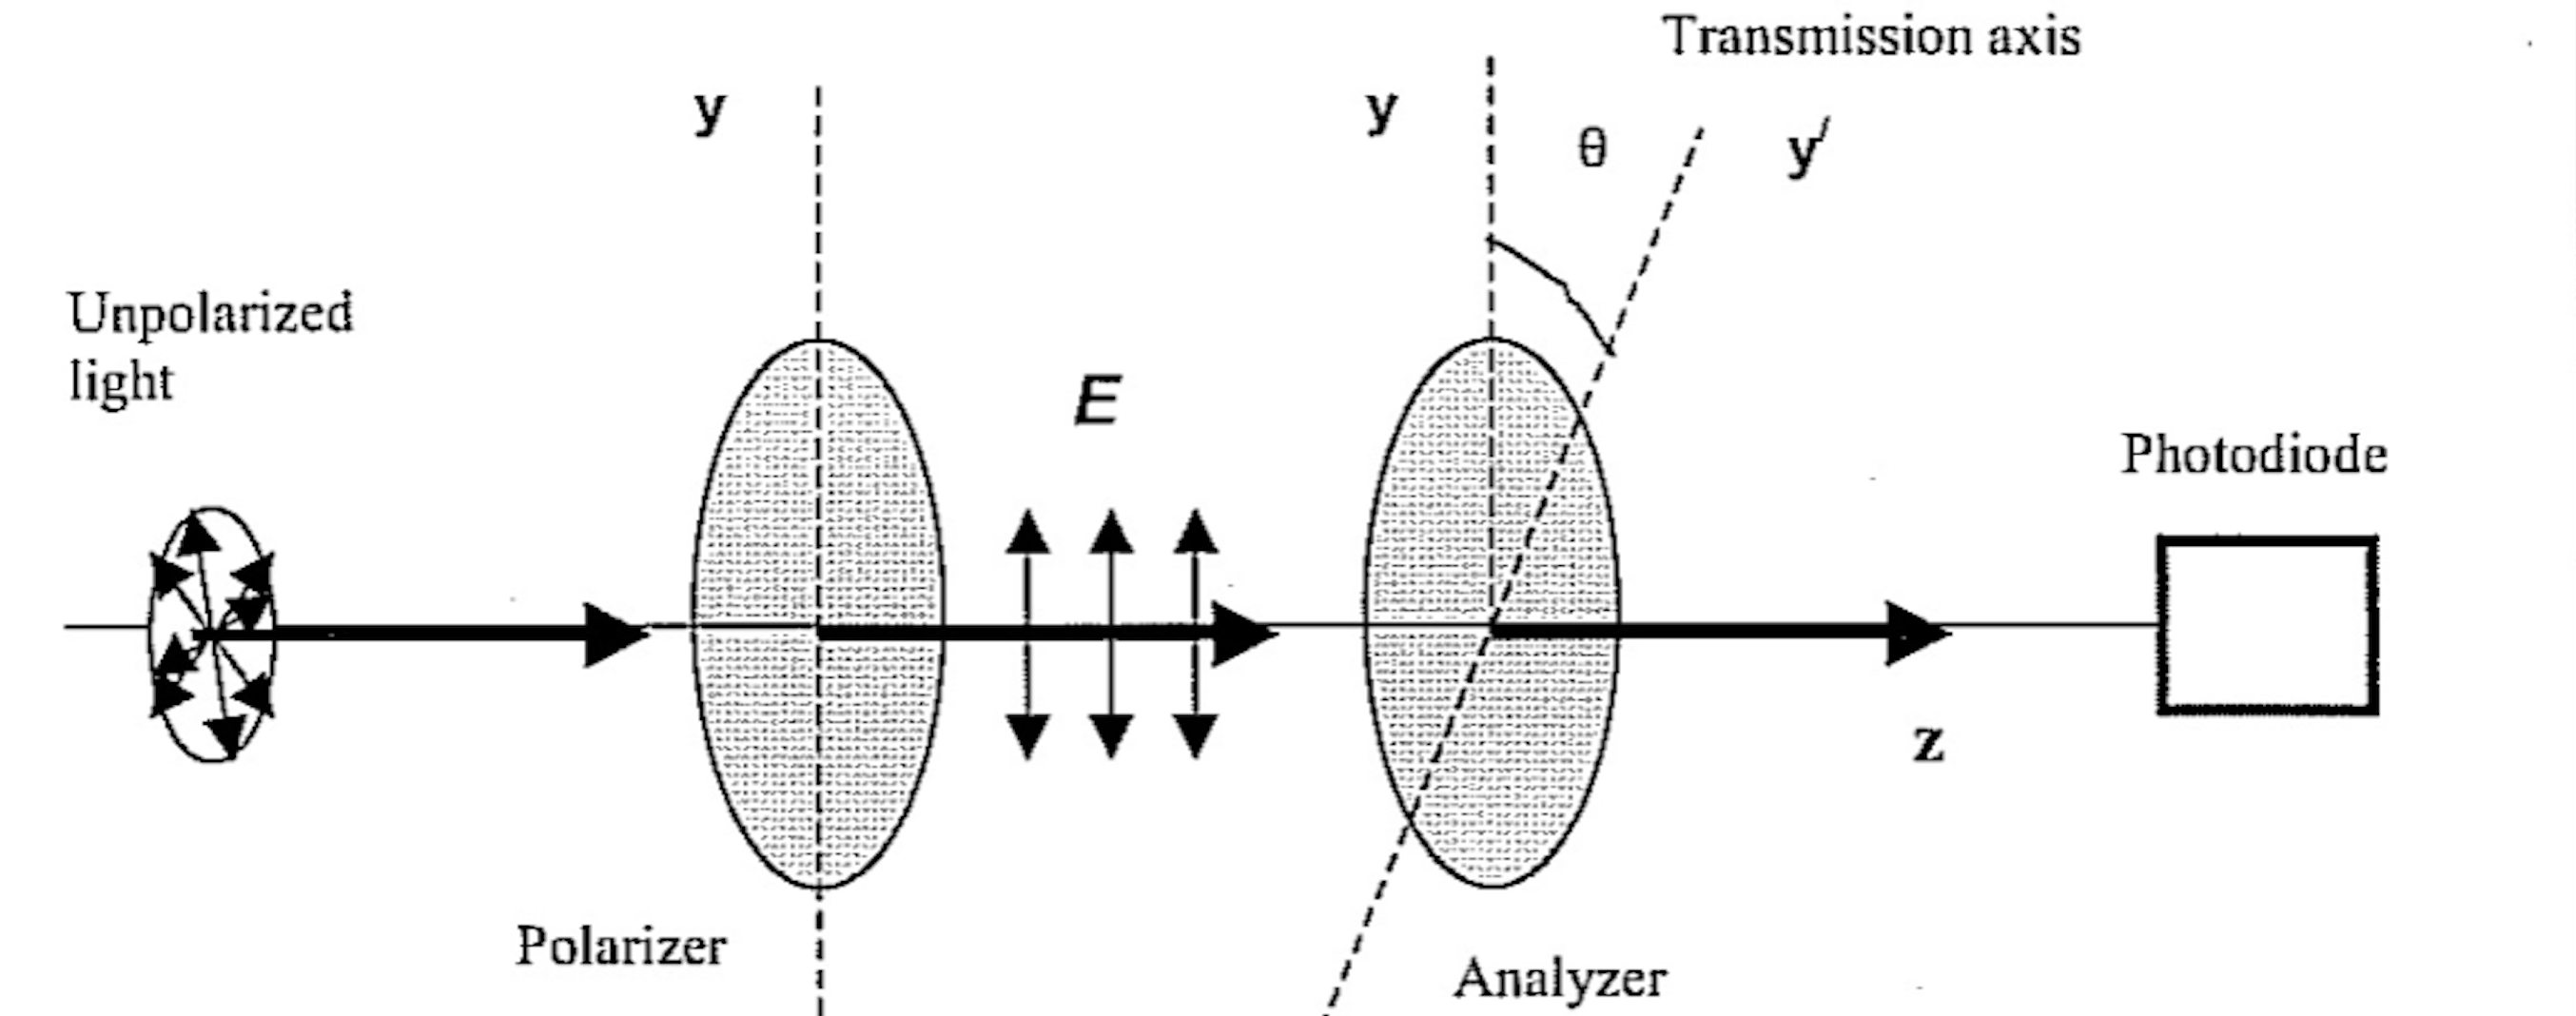
\includegraphics[width=\textwidth]{../figures/experimentOneApparatusA.png}
		\caption{\textbf{Figure 1: Apparatus for experiment 1 (two polarizers)}}
	\end{subfigure}\hfill
	\begin{subfigure}{0.45\textwidth}
		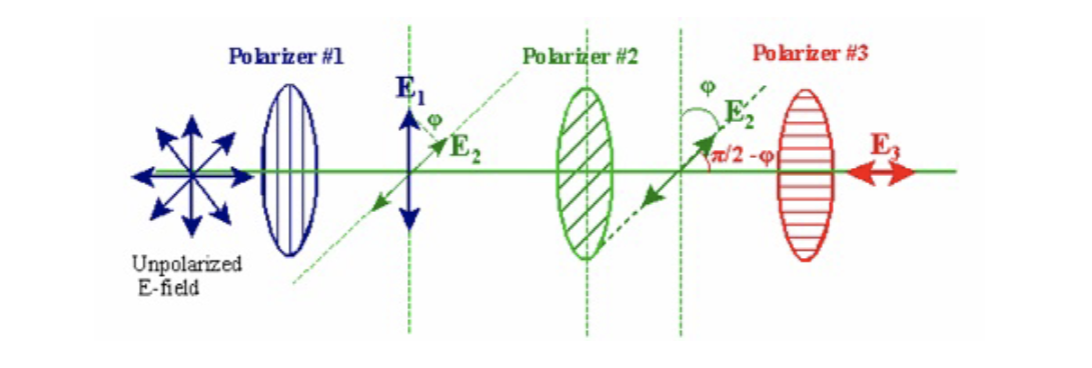
\includegraphics[width=\textwidth]{../figures/experimentOneApparatusB.png}
		\caption{\textbf{Figure 2: Apparatus for experiment 2 (three polarizers)}}
	\end{subfigure}
\end{figure}
\newpage
\textbf{Experiment 2}\\
A CI-6538 rotary motion sensor mounted on a spectrophotometer table, CI-6504A light sensor, Brewster's disk,
acrylic semicircular lens, two polarizers, a square polarizer and an optics track was set up as shown in \textbf{Figure 3}.
The second polarizer, which was further away from the laser, was rotated to 225 degrees and locked in place and the
Brewster's angle disk was zeroed. The Brewster's disk was then rotated to 120 degrees and the first polarizer,
closest to the laser, was rotated until the intensity detected was maximized. The data acquisition began without
using the square polarizer. To scan the light intensity versus angle, the spectrophotometer arm and Brewster's
disk were rotated clockwise at the same time, keeping the laser directed at the detector. This was repeated
multiple times until a set of consistent data was acquired. The same procedure was repeated, however, the
square polarizer on its horizontal axis was placed in front of the detector. Using the Brewster's Angle
application, the data was collected from light sensor and rotary motion sensor in volts and radians respectively.

\begin{figure}[H]
	\centering
	\begin{subfigure}{0.45\textwidth}
		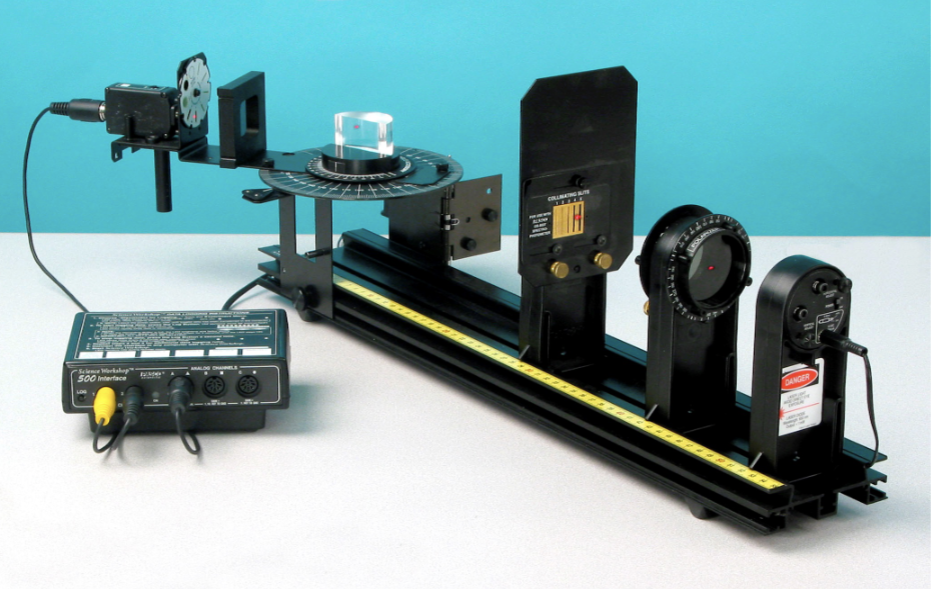
\includegraphics[width=\textwidth]{../figures/experimentTwoApparatus.png}
		\caption{\textbf{Figure 3: Apparatus for experiment 2}}
	\end{subfigure}
\end{figure}
\section{Results}
For both experiments, the uncertainty of the light intensity was taken to be $\pm 0.01 V$ as the value of the intensity would fluctuate
and the uncertainty of the angle was taken to be the resolution of the rotary motion sensor being
$\pm 0.00001rad$. \\

\textbf{Experiment 1}\\

To determine the initial intensity in the experimental setup with two polarizers, the model as defined
by \textbf{Equation 1} and implemented by \textbf{Function 1}, was passed into scipy's \lstinline{curve_fit} function and
fitted to the light intensity and angle data. The uncertainty of the initial intensity was determined
using \lstinline{curve_fit}'s covariance values since the diagonals of the covariance matrix represent
the variability of each parameter and the square root of this was taken to calculate the standard error.
\textbf{Figure 4} demonstrates the relationship between the angle of the polarizer with the rotary motion sensor
and the light intensity detected.\\
\textbf{Figure 5} demonstrates the relationship between the light intensity and the cosine of the angle squared.
To determine the uncertainty of the cosine of the angle squared, \textbf{Equation 2} was used to propagate the
uncertainty of the angle. Furthermore \textbf{Figures 6 and 7} picture the
residual plots for the relationship between the angle of the polarizer with the rotary motion sensor
and the light intensity detected and the relationship between the cosine of the polarizer with the
rotary motion sensor's angle squared and the light intensity detected respectively.

\begin{figure}[H]
	\begin{subfigure}{0.45\textwidth}
		\centering
		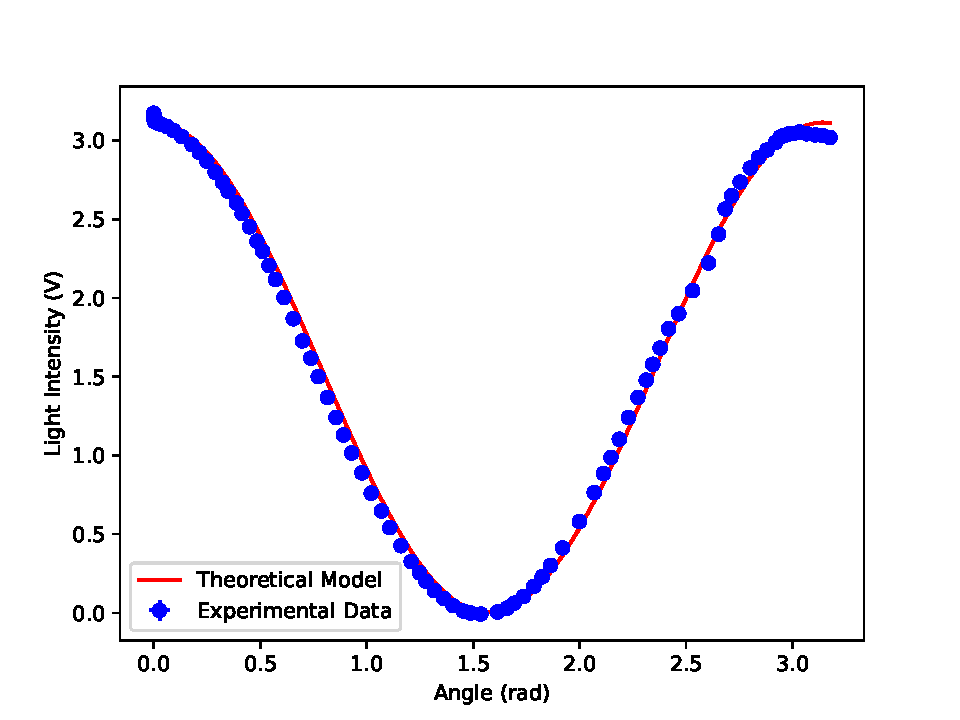
\includegraphics[width=\textwidth]{../figures/figure4.pdf}
		\caption{\textbf{Figure 4: Graph of detected intensity vs polarizer angle for the two polarizer system. Plot includes a regression fit of function 2. }}
	\end{subfigure}
	\hfill
	\begin{subfigure}{0.45\textwidth}
		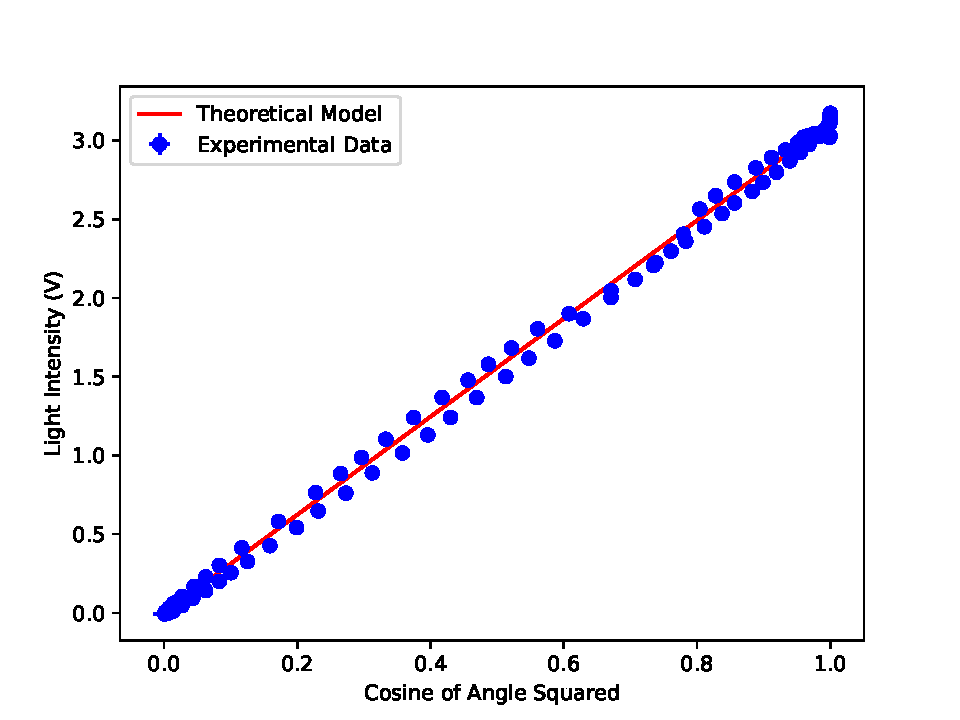
\includegraphics[width=\textwidth]{../figures/figure5.pdf}
		\caption{\textbf{Figure 5: Graph of detected intensity vs cos of the polarizer angle squared for the two polarizer system. Plot includes a regression fit of function 1.}}
	\end{subfigure}
	\begin{subfigure}{0.45\textwidth}
		\centering
		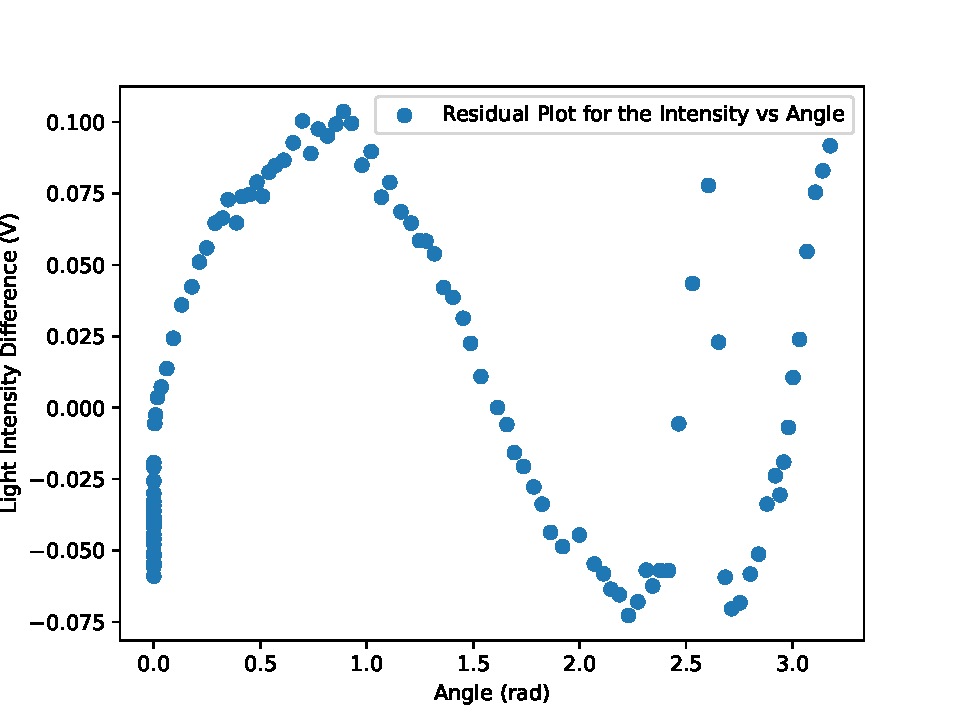
\includegraphics[width=\textwidth]{../figures/figure6.pdf}
		\caption{\textbf{Figure 6: Residuals plot for Figure 4.}}
	\end{subfigure}
	\hfill
	\begin{subfigure}{0.45\textwidth}
		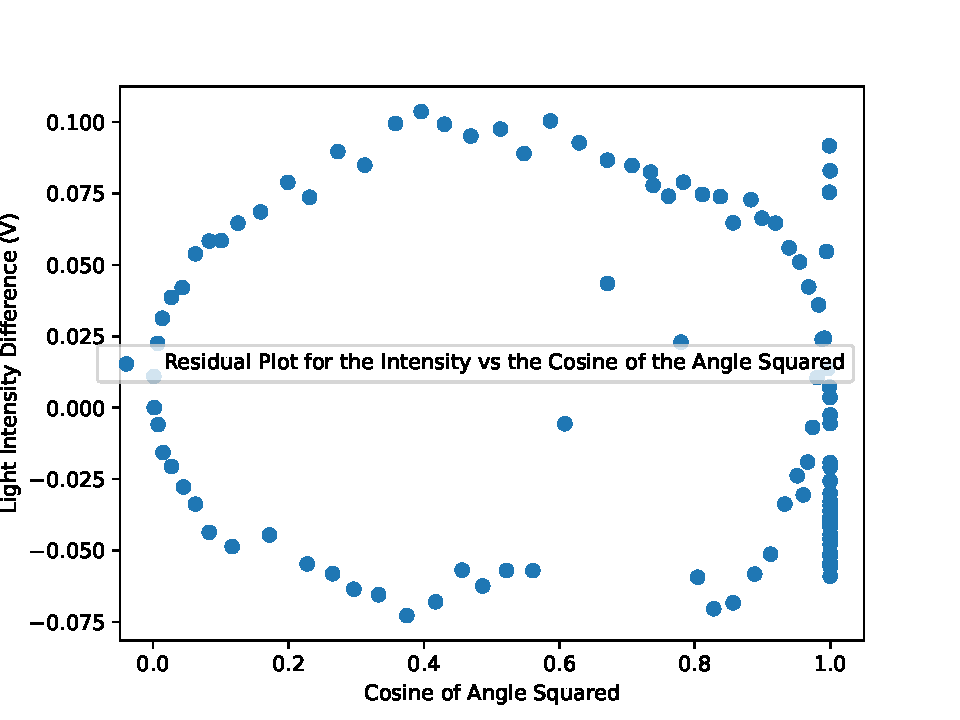
\includegraphics[width=\textwidth]{../figures/figure7.pdf}
		\caption{\textbf{Figure 7 : Residuals plot for Figure 5.}}
	\end{subfigure}
\end{figure}

To determine the light intensity passing through the first polarizer in the experimental setup with
three polarizers, the model as defined by \textbf{Equation 3}, where $\phi = \frac{\pi}{4} + \theta$ since the
angle difference between the two closest polarizers to the laser was $\frac{\pi}{4}$. This equation is
implemented by \textbf{Function 2}, which was passed into scipy's \lstinline{curve_fit} function and fitted
to the light intensity and angle data. The uncertainty of the
light intensity passing through the first polarizer was determined using \lstinline{curve_fit}'s
covariance using the same method as described above. \textbf{Figure 8} demonstrates the relationship between
the angle of the polarizer with the rotary motion sensor and the light intensity detected. Furthermore,
\textbf{Figure 9} pictures the residual plot for the relationship between the angle of the polarizer with the rotary
motion sensor and the light intensity detected.\\
\begin{figure}[H]
	\begin{subfigure}[t]{0.45\textwidth}
		\centering
		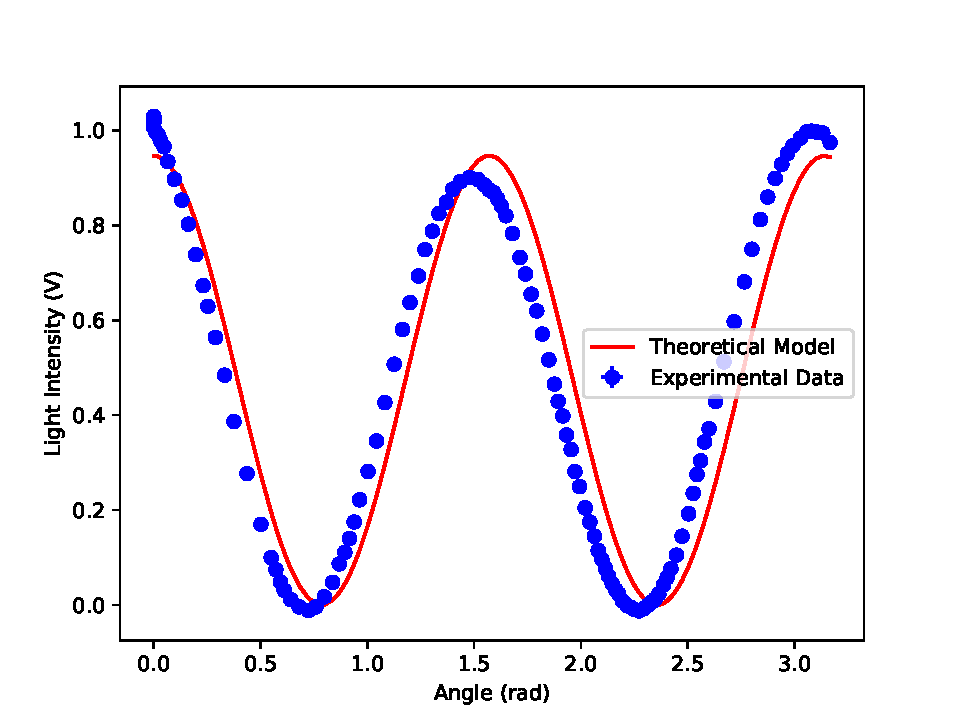
\includegraphics[width=\textwidth]{../figures/figure8.pdf}
		\caption{\textbf{Figure 8: Graph of detected intensity vs polarizer angle for the three polarizer system. Plot includes a regression fit of Function 2. }}
	\end{subfigure}
	\hfill
	\begin{subfigure}[t]{0.45\textwidth}
		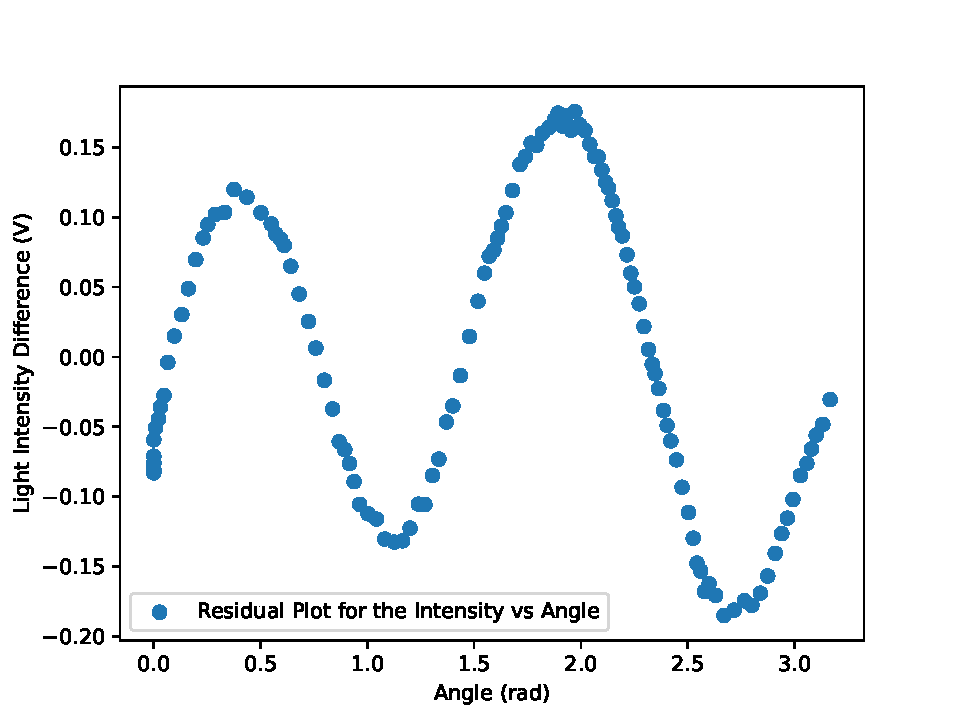
\includegraphics[width=\textwidth]{../figures/figure9.pdf}
		\caption{\textbf{Figure 9: Residuals plot for Figure 8}}
	\end{subfigure}
\end{figure}

The reduced chi-squared values were determined using \textbf{Function 3}. The values determined
for the initial intensity for the two polarizer setup and the intensity passing through the
first polarizer for three polarizer setup were $3.114 \pm 0.007V$ and $3.79 \pm 0.06V$ respectively.
Furthermore the angles at which the maximum and minimum light intensities are transmitted in the
three polarizer setup were determined to be $\frac{\pi}{4} + n\frac{\pi}{2}, n\in\mathbb{Z}$ and
$\frac{\pi}{2} + n\frac{\pi}{2} , n\in\mathbb{Z}$
respectively.\\


\textbf{Experiment 2}\\
At the start of every measurement interval, there was an initial angle of $180^\circ$.
The initial incidence angle was always set to $45^\circ$ at the start of each measurement
interval. The measured angle value was also increasing as the incidence angle decreased.
The combination of these factors meant that the measured angle values had to be scaled according
to the following equation:
$$\theta_{\rm incidence} = 180-\theta_{measured} + \phi_{initial}$$
Where $\phi_{\rm initial}$ is the initial incidence angle at the start of the measurements which was measured
to be $45^\circ$. This equation was applied to every value using its implementation (\textbf{Function 4})
(this function also converts all values to radians from degrees).\\

It was difficult to get a complete measurement of all angles without the laser beam occasionally
missing the detector. This meant that there were significant portions of the data that were
missing intervals. Due to this \textbf{Function 5} was built to reduce the problematic points.
This resulted in a noticeable drop in points where intensity dropped significantly. \textbf{Figure 10}
shows a graph of the ratio of the polarized to non-polarized intensity measurements before
problematic points had been removed. \textbf{Figure 11} shows the same data after this procedure was performed.
\begin{figure}[H]
	\begin{subfigure}{0.45\textwidth}
		\centering
		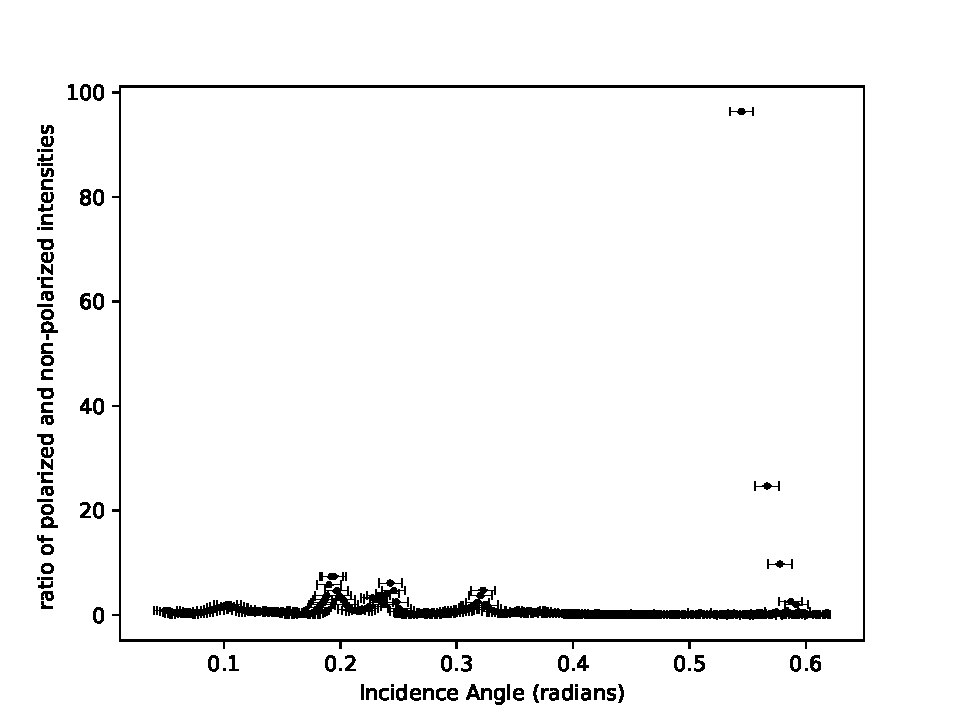
\includegraphics[width=\textwidth]{../figures/figure10.pdf}
		\caption{\textbf{Figure 10: Graph of polarized intensity over non-polarized intensity ratio vs incidence angle before the data cleanup was performed.}}
	\end{subfigure}
	\hfill
	\begin{subfigure}{0.45\textwidth}
		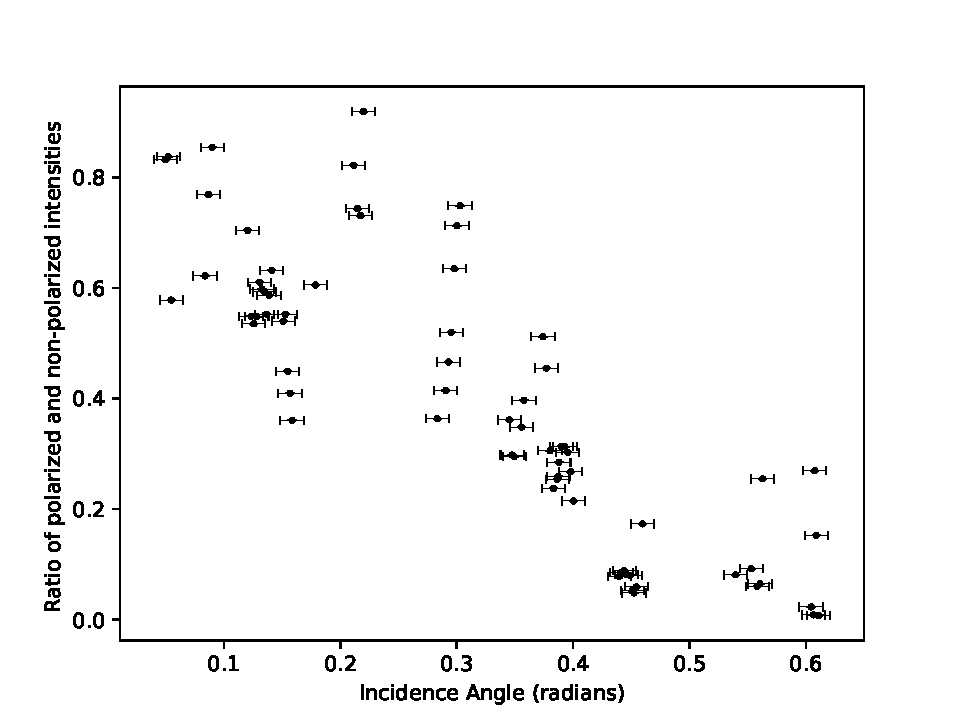
\includegraphics[width=\textwidth]{../figures/figure11.pdf}
		\caption{\textbf{Figure 11: Graph of polarized intensity over non-polarized intensity ratio vs incidence angle after the data cleanup was performed.}}
	\end{subfigure}
\end{figure}
The effect of this change is also clearly visible in the plots of both intensities:
\begin{figure}[H]
	\begin{subfigure}{0.45\textwidth}
		\centering
		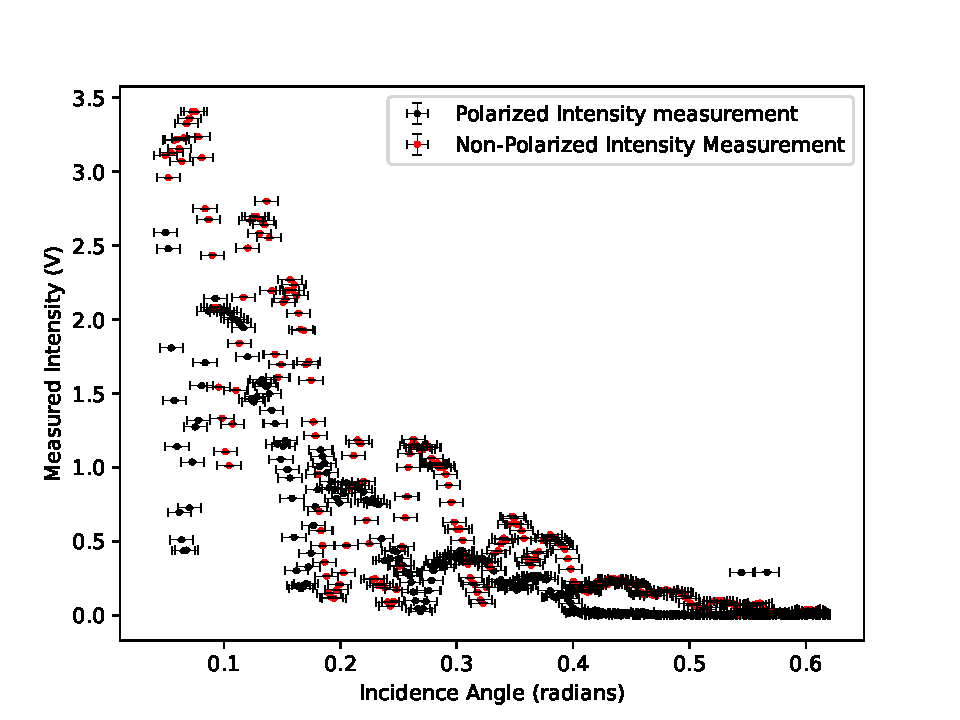
\includegraphics[width=\textwidth]{../figures/figure12.pdf}
		\caption{\textbf{Figure 12: Graph of raw intensity measurements vs incidence angle of both polarized and non-polarized measurements before data cleanup was done. }}
	\end{subfigure}
	\hfill
	\begin{subfigure}{0.45\textwidth}
		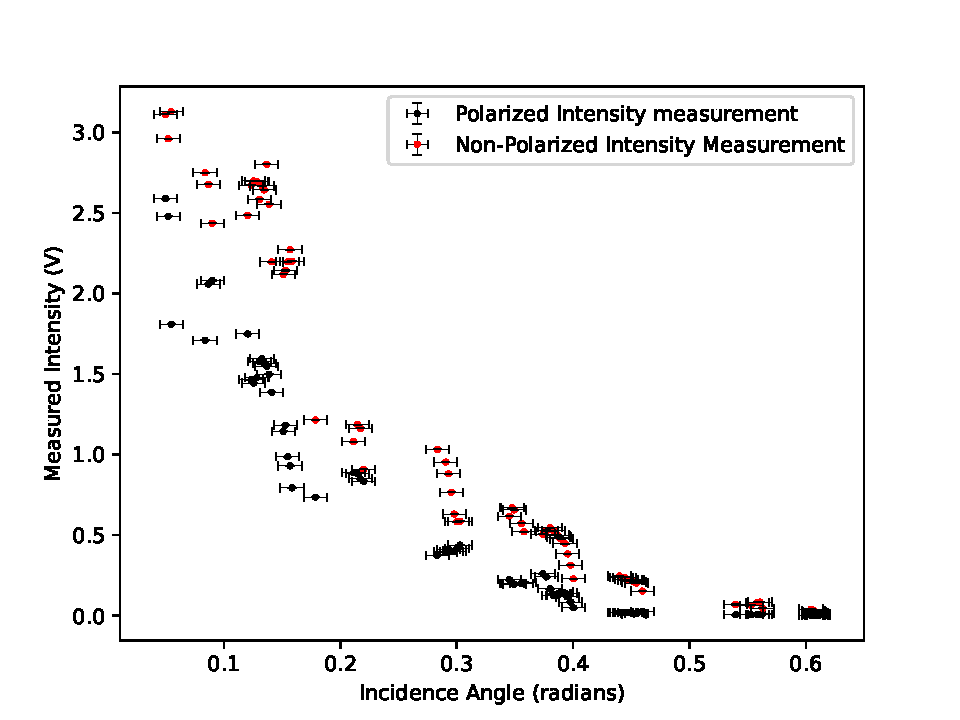
\includegraphics[width=\textwidth]{../figures/figure13.pdf}
		\caption{\textbf{Figure 13: Graph of raw intensity measurements vs incidence angle of both polarized and non-polarized measurements before data cleanup was done.}}
	\end{subfigure}
\end{figure}
The function takes every data points and compares it to the average of the 5 data points before it. It removes the
point if it is less than 90 percent of the average.\\

The Brewster's angle was calculated as the minimum of the ratio of reflected
horizontally polarized intensity over the reflected intensity. The computed Brewster's Angle was: $0.61\pm0.01$ radians.
This value was used in conjunction with \textbf{Equation 6} to calculate the refractive index of acrylic ($n_2$).
The calculated value for $n_2$ was $0.70\pm0.02$.\\
\newpage
These values were used in conjunction with \textbf{Equation 7} and \textbf{Equation 8} to calculate the perpendicular
and parallel reflection coefficients for the system at each angle. These values are modelled in \textbf{Figure 14}
In practice, this was done in python using the implementations of \textbf{Equations 7 and 8}: \textbf{Functions 6 and 7}.
\begin{figure}[H]
	\centering
	\begin{subfigure}{0.45\textwidth}
		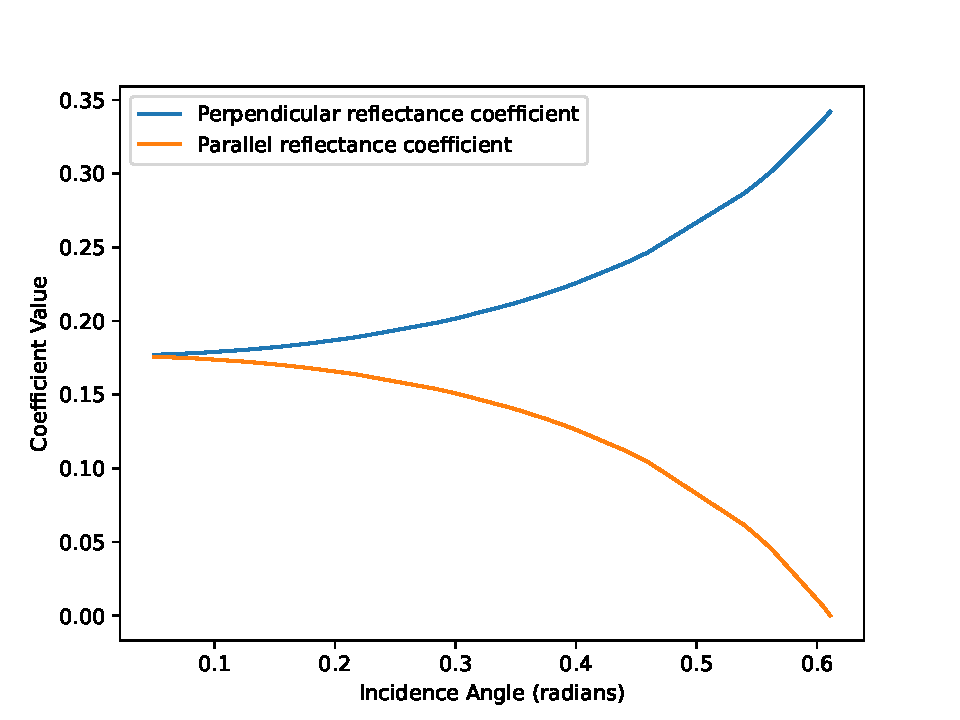
\includegraphics[width=\textwidth]{../figures/figure14.pdf}
		\caption{\textbf{Figure 14: Parallel and perpendicular reflection coefficients for the air acrylic system vs incidence angle}}
	\end{subfigure}
\end{figure}
There were two compromises that had to be made during these calculations. The first is
that the polarized and non-polarized ($I$ and $I_0$) data sets had different angle values
for their corresponding measurements. They were close to each other but not exactly the same.
For the purpose of this experiment, due to the proximity of the measured angles, the ratio
was approximated by dividing identical indexes in each data set by each other. Additionally,
the range of the intensity detector was not sufficient to get a full range of values.
A subset of both data sets had to be removed from the calculations due to the detector
reaching its maximum measurable intensity. Both of these compromises are discussed further
in the analysis and discussion section.

\section{Analysis and Discussion}
The initial intensity of the light in the experimental setup with two polarizers is $3.114 \pm 0.007 V$ and the intensity
of the light passing through the first polarizer in the experimental setup with three polarizers is $3.79 \pm 0.06 V$.

Examining \textbf{Figures 4 and 8},the graph for two polarizers depicts a sinusoid of period $\pi$ while the
graph for three polarizers covers two periods where the period of the sinusoid is $\frac{\pi}{2}$.
The amplitude of the sinusoid pictured by the graph for two polarizers is also roughly three times greater
in magnitude than the amplitude of the sinusoid pictured by the graph for three polarizers. In regards
to the amplitudes, it is expected that the amplitude of the sinusoid pictured in \textbf{Figure 8} would be less than the amplitude
of \textbf{Figure 4}'s sinusoid as the light must pass through three polarizers instead of two, limiting the amount of light which
was transmitted. \textbf{Figure 5} demonstrates a linear relationship as expected which is described by $I(\theta) = I_0C(\theta)$ where $C(\theta) = \cos^2\theta$.
Analyzing \textbf{Figure 8} and taking into account that the initial difference between the first polarizer and the
polarizer with the rotary motion sensor was $\frac{\pi}{4}$, the maxima and minima for the three polarizer experiment occur when the
angle between the first polarizer and the polarizer with the rotary motion sensor is $\frac{\pi}{4} + n\frac{\pi}{2}, n\in \mathbb{Z}$
and $\frac{\pi}{2}+n\frac{\pi}{2}, n\in\mathbb{Z}$ respectively.\\

The respective reduced chi-squared values were determined to be $32.4$ and $113.3$. Visually, the models fit the experimental
data relatively well, however the reduced chi-squared value, $32.4$, determined for two polarizers indicates that the uncertainty
of the light intensity may have been underestimated. Examining \textbf{Figure 8}, the theoretical model is shifted slightly to the
right of the experimental data, in turn this is reflected in the reduced chi-squared value of $113.3$.\\

\textbf{Experiment 2}\\
The calculated value for $\theta_p$ was $0.61\pm 0.01$ this was significantly different to the literature value of
approximately $1.5$. There were multiple significant sources of error in this experiment that likely lead to
these less accurate results. \\

As discussed in the results section, the detector that was used in this experiment had a range that was not sufficient to measure
the full range of intensities across all values. The first polarizer adjustment was done to reduce the
intensity to a point where the detector was not maxed out through most of its range. There was still a subset
towards the end in both data sets that was at a constant max value. Using a detector with a wider
range of intensity values would likely solve this issue.\\

The two data sets had differing increments of angle measurements. This resulted in a compromise having to be
made when taking the ratio of the two data sets, likely leading to less accurate results. Ideally, the
incidence angles of each intensity measurement should be the same across both data sets. Setting up the
computer to record intensities at set angle intervals would eliminate this issue.\\

While the lab was being performed, there was difficulty keeping the laser beam lined up with the detector.
This can be clearly seen in \textbf{Figures 10 and 12}, which plot data that has not been programmatically cleaned up.
The data set had certain intervals that were $\approx 0$ intensity due to this. This was partially
mitigated by the data cleanup algorithm shown in \textbf{Function 5}, but it wasn't completely successful.
Ensuring that the laser beam is lined up with the detector through the entire range of measurements
could be achieved through a gear ratio or similar setup that would rotate both the acrylic lens and detector
arm at the ideal ratio to maintain alignment. This would result in more representative data that
wouldn't have to be cleaned up programmatically.\\

In the results, the proximity of the calculated Brewster's angle to the maximum measured angle
incidencce angle is notable. The maximum measured incidence angle was approximately $0.61\pm0.01rad$
and the calculated Brewster's angle value was $0.61\pm0.01rad$. Additionally, in \textbf{Figure 11} there is a
clear decrease in intensity for higher angles. It is possible that this trend would've continued to larger
incidence angles. Therefore, for a conclusive Brewster's angle measurement, a larger range of angles would
confirm whether the calculated Brewster's angle was correct. Ideally, for a future experiment, measurements
should start with the beam as close as possible to perpendicular to the surface of the lens.\\

The $n_2$ value for water is approximately $1.3$ and the acrylic refractive index is approximately $1.5$ Considering that the
$n_1$ value would remain the same as the first medium is still air, if the beam was to reflect off of a
water surface then there would be a decrease in Brewster's due to the relation $\tan(\theta_p) = \frac{n2}{n1}$. If the
data was to be measured with a vertical polarizer, the ratio graph would likely be inverted due to the fact that a high portion
of the total light being horizontally polarized will result in a low vertically polarized component and vice-versa. Polarized sunglasses
are vertically polarized. Since most of the glare that will be seen outdoors is reflection off of the water or ground, the
horizontal polarized light will make up a higher portion of the visible light. This could be verified by running the laser through
a horizontal polarizer to ensure horizontally polarized light and then rotating the sunglasses from their normal axis to $90^\circ$
in one direction and measuring the intensity.

\section{Conclusion}
\textbf{Experiment 1}\\
In regards to the experimental setup with two polarizers, the theoretical depicted in \textbf{Figure 4} model visually fits the data relatively well,
verifying that the light intensity passing through a polarizer can be quantified using Malus' Law. Furthermore in the
experimental setup with three polarizers, the maxima and minima of the experimental data occur roughly near the maxima
and minima of the theoretical model, verifying that the maxima and minima occur when the angle between the first polarizer
and the polarizer with the rotary motion sensor is $\frac{\pi}{4} + n\frac{\pi}{2}$ where $n \in \mathbb{Z}$ and
$\frac{\pi}{2}+n\frac{\pi}{2}$ where $n\in \mathbb{Z}$ respectively.\\

\textbf{Experiment 2}\\
There were numerous issues with the data that was acquired in this experiment that lead to calculated values that are
likely not accurate as discussed in the Analysis and Discussion section. To get conclusive results, the experiment should be
repeated with the improvements discussed in the analysis section. This would result in a measurement
of Brewster's angle that would be much more accurate.
\newpage
\section{Appendix}
{\large\textbf{Equations}}\\
\begin{tabular}{p{0.45\linewidth} p{0.45\linewidth}}
	$$I(\theta) = I_0\cos^2(\theta)$$
	\begin{center}
		\textbf{Equation 1: Malus' Law}
	\end{center}
	&
	$$u(\cos^2(x)) = \frac{2\left|\sin(x) \times u(x)\right|}{\cos^2(x)}$$
	\begin{center}
		\textbf{Equation 2: Cos-Squared propagation}
	\end{center}
	\\
	$$I_3 = \frac{I_1}4\sin^2(2\phi) $$
	\begin{center}
		\textbf{Equation 3: Relation between first and third polarizer intensities}
	\end{center}
	&
	$$\chi^2_R = \frac{1}{N-n}\sum_{i=1}^N\left(\frac{y_i-y(x_i)}{u(y_i)}\right)$$
	\begin{center}
		\textbf{Equation 4: Reduced chi-Squared Metric}
	\end{center}\\
	% Begin experiment 2
	$$ \frac{\sin(\theta_2)}{\sin(\theta_1)} = \frac{n_1}{n_2} \iff \theta_2 = \arcsin\left(\frac{n_2\sin(\theta_1)}{n_1}\right)  $$
	\begin{center}
		\textbf{Equation 5: Snell's Law}
	\end{center}
	&
	$$\tan\theta_p = \frac{n_2}{n_1} \iff \theta_p = \arctan{\frac{n_2}{n_1}}$$
	\begin{center}
		\textbf{Equation 6: Brewster's Angle definition}
	\end{center}\\

	$$ r_\parallel = \frac{n_1\cos\theta_2 - n_2\cos\theta_1}{n_1\cos\theta_2 + n_2\cos\theta_1}$$
	\begin{center}
		\textbf{Equation 7: Parallel reflectance Fresnel equation}
	\end{center}
	&
	$$r_\perp = \frac{n_1\cos\theta_1 - n_2\cos\theta_2}{n_1\cos\theta_1 + n_2\cos\theta_2}$$
	\begin{center}
		\textbf{Equation 8: Perpendicular reflectance Fresnel equation}
	\end{center}\\

	$$u(\arctan(x)) = \sqrt{\left(\frac{\partial \arctan(x)}{\partial x}\right)^2 \left(u(x)\right)^2} = \frac{u(x)}{1+x^2}$$
	\begin{center}
		\textbf{Equation 9: $\arctan$ error propagation}
	\end{center}
	&
	$$u(\tan(x)) = \sqrt{\left(\frac{\partial \tan(x)}{\partial x}\right)^2 \left(u(x)\right)^2} = \frac{u(x)}{\cos^2(x)}$$
	\begin{center}
		\textbf{Equation 10: $\tan$ error propagation}
	\end{center}\\

\end{tabular}
\newpage
{\large\textbf{Functions}}\\
\begin{verbatim}
def cosineModel(angle, initialIntensity):
    return initialIntensity * ((np.cos(angle)) ** 2)
\end{verbatim}
\begin{center}
	\textbf{Function 1: Cosine Model (implements Equation 1)}\\
\end{center}
\begin{verbatim}
def intensity(angle, firstIntensity):
    return firstIntensity / 4 * (np.sin(np.pi / 2 + 2 * angle) ** 2)
\end{verbatim}
\begin{center}
	\textbf{Function 2: Intensity Model (implements Equation 3)}\\
\end{center}
\begin{verbatim}
def characterize(y: any, func: any, u: any) -> float:
    """Return the chi^2 metric to determine how well a model function fits a
    given set of data using the measured data <y>, the prediction with the model
    <func> and the uncertainty on each measurement's dependent data <u>.
    """
    value = 0

    for i in range(np.size(y)):
        value += ((y[i] - func[i]) ** 2) / (u ** 2)
        i += 1

    return value / (np.size(y) - 1)
\end{verbatim}
\begin{center}
	\textbf{Function 3: Reduced chi-squared metric (implements Equation 4)}
\end{center}
\begin{verbatim}
def convertMeasuredToIncidence(measurement):
    return np.radians(180 - measurement + 35)
\end{verbatim}
\begin{center}
	\textbf{Function 4: Function used to convert measured angles into incidence angles in radians}
\end{center}
\newpage
\begin{verbatim}
	def removeInconsistentPoints(firstIntensities, secondIntensities, thetas):
    i = 5
    while i < len(firstIntensities):
        firstIntensitiesAvg = np.sum(firstIntensities[i - 5 : i]) / 5
        secondIntensitiesAvg = np.sum(secondIntensities[i - 5 : i]) / 5
        if (
            firstIntensities[i] - firstIntensitiesAvg
            < -firstIntensitiesAvg / 10
        ) or (
            secondIntensities[i] - secondIntensitiesAvg
            < -secondIntensitiesAvg / 10
        ):

            firstIntensities = np.delete(firstIntensities, i)
            secondIntensities = np.delete(secondIntensities, i)

            thetas = np.delete(thetas, i)
            break
        i += 1
    else:
        return firstIntensities, secondIntensities, thetas

    firstIntensities, secondIntensities, thetas = removeInconsistentPoints(
        firstIntensities, secondIntensities, thetas
    )
    return firstIntensities, secondIntensities, thetas


\end{verbatim}
\begin{center}
	\textbf{Function 5: Function used to remove problematic data points}
\end{center}


\begin{verbatim}
def parallelReflectanceCoeffModel(theta1, theta2, n2):
    """
        Model used to calculate parallel reflectance coefficient.
        Based off of fresnels equation.
        Uses a n1 value of 1 for the air.
        <n2> (index of refraction for acrylic) is theoretically calculated with
            Brewster's angle
        <theta1> (angle of incidence) is experimentally measured
        <theta2> (angle of reflectance) is determined theoretically with snells
            law
    """
    return (np.cos(theta2) - n2 * np.cos(theta1)) / (
        np.cos(theta2) + n2 * np.cos(theta1)
    )

\end{verbatim}
\begin{center}
	\textbf{Function 6: Fresnel's parallel reflectance coefficient equation python model}\\

\end{center}

\begin{verbatim}
def perpendicularReflectanceCoeffModel(theta1, theta2, n2):
    """
        Model used to calculate perpendicular reflectance coefficient.
        Based off of fresnels equation.
        Uses a n1 value of 1 for the air.
        <n2> (index of refraction for acrylic) is theoretically calculated with
            Brewster's angle
        <theta1> (angle of incidence) is experimentally measured
        <theta2> (angle of reflectance) is determined theoretically with snells
            law
    """
    return (np.cos(theta1) - n2 * np.cos(theta2)) / (
        np.cos(theta1) + n2 * np.cos(theta2)
    )
\end{verbatim}
\begin{center}
	\textbf{Function 7: Fresnel's perpendicular reflectance coefficient equation python model}
\end{center}
{\large\textbf{Raw Experimental Data}}\\
\begin{center}
	\textbf{Results for Experiment One (two-polarizer setup)}
\end{center}
\begin{tabular}{| p{0.21\textwidth} | p{0.21\textwidth} |}
\hline
Incidence Angle (radians) & Measured Intensity (V)\\
\hline
$0.0 \pm 0.01$ & $3.1525 \pm 0.0001$\\
$0.0 \pm 0.01$ & $3.1525 \pm 0.0001$\\
$0.0 \pm 0.01$ & $3.15491 \pm 0.0001$\\
$0.0 \pm 0.01$ & $3.14444 \pm 0.0001$\\
$0.0 \pm 0.01$ & $3.14718 \pm 0.0001$\\
$0.0 \pm 0.01$ & $3.15266 \pm 0.0001$\\
$0.0 \pm 0.01$ & $3.1504 \pm 0.0001$\\
$0.0 \pm 0.01$ & $3.15459 \pm 0.0001$\\
$0.0 \pm 0.01$ & $3.15089 \pm 0.0001$\\
$0.0 \pm 0.01$ & $3.1562 \pm 0.0001$\\
$0.0 \pm 0.01$ & $3.15363 \pm 0.0001$\\
$0.0 \pm 0.01$ & $3.16039 \pm 0.0001$\\
$0.0 \pm 0.01$ & $3.16232 \pm 0.0001$\\
$0.0 \pm 0.01$ & $3.16538 \pm 0.0001$\\
$0.0 \pm 0.01$ & $3.17344 \pm 0.0001$\\
$0.0 \pm 0.01$ & $3.17006 \pm 0.0001$\\
$0.0 \pm 0.01$ & $3.16635 \pm 0.0001$\\
$0.0 \pm 0.01$ & $3.16571 \pm 0.0001$\\
$0.0 \pm 0.01$ & $3.1699 \pm 0.0001$\\
$0.0 \pm 0.01$ & $3.16877 \pm 0.0001$\\
$0.0 \pm 0.01$ & $3.16603 \pm 0.0001$\\
$0.0 \pm 0.01$ & $3.16538 \pm 0.0001$\\
$0.0 \pm 0.01$ & $3.16571 \pm 0.0001$\\
$0.0 \pm 0.01$ & $3.15878 \pm 0.0001$\\
$0.0 \pm 0.01$ & $3.14879 \pm 0.0001$\\
$0.0 \pm 0.01$ & $3.14009 \pm 0.0001$\\
$0.0 \pm 0.01$ & $3.13365 \pm 0.0001$\\
$0.0 \pm 0.01$ & $3.13526 \pm 0.0001$\\
$0.0 \pm 0.01$ & $3.11996 \pm 0.0001$\\
$0.01 \pm 0.01$ & $3.11674 \pm 0.0001$\\
$0.02 \pm 0.01$ & $3.10997 \pm 0.0001$\\
$0.03 \pm 0.01$ & $3.10337 \pm 0.0001$\\
\hline
\end{tabular}\hfill
\begin{tabular}{| p{0.21\textwidth} | p{0.21\textwidth} |}
\hline
Incidence Angle (radians) & Measured Intensity (V)\\
\hline
$0.09 \pm 0.01$ & $3.06406 \pm 0.0001$\\
$0.13 \pm 0.01$ & $3.0254 \pm 0.0001$\\
$0.18 \pm 0.01$ & $2.97353 \pm 0.0001$\\
$0.21 \pm 0.01$ & $2.92327 \pm 0.0001$\\
$0.25 \pm 0.01$ & $2.86979 \pm 0.0001$\\
$0.29 \pm 0.01$ & $2.7986 \pm 0.0001$\\
$0.32 \pm 0.01$ & $2.73448 \pm 0.0001$\\
$0.35 \pm 0.01$ & $2.6773 \pm 0.0001$\\
$0.39 \pm 0.01$ & $2.6032 \pm 0.0001$\\
$0.41 \pm 0.01$ & $2.53538 \pm 0.0001$\\
$0.45 \pm 0.01$ & $2.45194 \pm 0.0001$\\
$0.48 \pm 0.01$ & $2.36029 \pm 0.0001$\\
$0.51 \pm 0.01$ & $2.29682 \pm 0.0001$\\
$0.54 \pm 0.01$ & $2.20581 \pm 0.0001$\\
$0.57 \pm 0.01$ & $2.11818 \pm 0.0001$\\
$0.61 \pm 0.01$ & $2.00316 \pm 0.0001$\\
$0.65 \pm 0.01$ & $1.86753 \pm 0.0001$\\
$0.7 \pm 0.01$ & $1.72723 \pm 0.0001$\\
$0.74 \pm 0.01$ & $1.61753 \pm 0.0001$\\
$0.77 \pm 0.01$ & $1.50043 \pm 0.0001$\\
$0.82 \pm 0.01$ & $1.36705 \pm 0.0001$\\
$0.86 \pm 0.01$ & $1.24124 \pm 0.0001$\\
$0.89 \pm 0.01$ & $1.12978 \pm 0.0001$\\
$0.93 \pm 0.01$ & $1.01541 \pm 0.0001$\\
$0.98 \pm 0.01$ & $0.88896 \pm 0.0001$\\
$1.02 \pm 0.01$ & $0.76058 \pm 0.0001$\\
$1.07 \pm 0.01$ & $0.64685 \pm 0.0001$\\
$1.11 \pm 0.01$ & $0.54118 \pm 0.0001$\\
$1.16 \pm 0.01$ & $0.42665 \pm 0.0001$\\
$1.21 \pm 0.01$ & $0.3263 \pm 0.0001$\\
$1.25 \pm 0.01$ & $0.2551 \pm 0.0001$\\
\hline
\end{tabular}\\
\begin{tabular}{| p{0.21\textwidth} | p{0.21\textwidth} |}
\hline
Incidence Angle (radians) & Measured Intensity (V)\\
\hline
$1.32 \pm 0.01$ & $0.14138 \pm 0.0001$\\
$1.36 \pm 0.01$ & $0.09257 \pm 0.0001$\\
$1.4 \pm 0.01$ & $0.04618 \pm 0.0001$\\
$1.45 \pm 0.01$ & $0.01171 \pm 0.0001$\\
$1.49 \pm 0.01$ & $-0.00118 \pm 0.0001$\\
$1.54 \pm 0.01$ & $-0.00714 \pm 0.0001$\\
$1.61 \pm 0.01$ & $0.00591 \pm 0.0001$\\
$1.66 \pm 0.01$ & $0.02959 \pm 0.0001$\\
$1.69 \pm 0.01$ & $0.06197 \pm 0.0001$\\
$1.74 \pm 0.01$ & $0.10546 \pm 0.0001$\\
$1.78 \pm 0.01$ & $0.16796 \pm 0.0001$\\
$1.82 \pm 0.01$ & $0.22901 \pm 0.0001$\\
$1.86 \pm 0.01$ & $0.3023 \pm 0.0001$\\
$1.92 \pm 0.01$ & $0.41296 \pm 0.0001$\\
$2.0 \pm 0.01$ & $0.58016 \pm 0.0001$\\
$2.07 \pm 0.01$ & $0.7638 \pm 0.0001$\\
$2.11 \pm 0.01$ & $0.88429 \pm 0.0001$\\
$2.15 \pm 0.01$ & $0.98738 \pm 0.0001$\\
$2.19 \pm 0.01$ & $1.10288 \pm 0.0001$\\
$2.23 \pm 0.01$ & $1.24012 \pm 0.0001$\\
$2.27 \pm 0.01$ & $1.36818 \pm 0.0001$\\
$2.31 \pm 0.01$ & $1.47836 \pm 0.0001$\\
$2.34 \pm 0.01$ & $1.57887 \pm 0.0001$\\
$2.38 \pm 0.01$ & $1.68213 \pm 0.0001$\\
$2.42 \pm 0.01$ & $1.80407 \pm 0.0001$\\
$2.47 \pm 0.01$ & $1.89991 \pm 0.0001$\\
$2.53 \pm 0.01$ & $2.04634 \pm 0.0001$\\
$2.6 \pm 0.01$ & $2.2224 \pm 0.0001$\\
$2.65 \pm 0.01$ & $2.40507 \pm 0.0001$\\
$2.68 \pm 0.01$ & $2.56454 \pm 0.0001$\\
$2.71 \pm 0.01$ & $2.64927 \pm 0.0001$\\
\hline
\end{tabular}\hfill
\begin{tabular}{| p{0.21\textwidth} | p{0.21\textwidth} |}
\hline
Incidence Angle (radians) & Measured Intensity (V)\\
\hline
$2.8 \pm 0.01$ & $2.82566 \pm 0.0001$\\
$2.84 \pm 0.01$ & $2.89186 \pm 0.0001$\\
$2.88 \pm 0.01$ & $2.93954 \pm 0.0001$\\
$2.92 \pm 0.01$ & $2.98658 \pm 0.0001$\\
$2.94 \pm 0.01$ & $3.02121 \pm 0.0001$\\
$2.96 \pm 0.01$ & $3.03007 \pm 0.0001$\\
$2.98 \pm 0.01$ & $3.04087 \pm 0.0001$\\
$3.0 \pm 0.01$ & $3.0436 \pm 0.0001$\\
$3.03 \pm 0.01$ & $3.05359 \pm 0.0001$\\
$3.07 \pm 0.01$ & $3.04264 \pm 0.0001$\\
$3.11 \pm 0.01$ & $3.03523 \pm 0.0001$\\
$3.14 \pm 0.01$ & $3.03152 \pm 0.0001$\\
$3.18 \pm 0.01$ & $3.01896 \pm 0.0001$\\
\hline
\end{tabular}

\begin{tabular}{| p{0.21\textwidth} | p{0.21\textwidth} |}
\hline
Incidence Angle (radians) & Measured Intensity (V)\\
\hline
$0.0 \pm 0.01$ & $1.02878 \pm 0.0001$\\
$0.0 \pm 0.01$ & $1.02733 \pm 0.0001$\\
$0.0 \pm 0.01$ & $1.02701 \pm 0.0001$\\
$0.0 \pm 0.01$ & $1.02749 \pm 0.0001$\\
$0.0 \pm 0.01$ & $1.02233 \pm 0.0001$\\
$0.0 \pm 0.01$ & $1.0175 \pm 0.0001$\\
$0.0 \pm 0.01$ & $1.00574 \pm 0.0001$\\
$0.01 \pm 0.01$ & $0.99688 \pm 0.0001$\\
$0.02 \pm 0.01$ & $0.98915 \pm 0.0001$\\
$0.03 \pm 0.01$ & $0.97884 \pm 0.0001$\\
$0.05 \pm 0.01$ & $0.96531 \pm 0.0001$\\
$0.07 \pm 0.01$ & $0.93422 \pm 0.0001$\\
$0.1 \pm 0.01$ & $0.89701 \pm 0.0001$\\
$0.13 \pm 0.01$ & $0.85272 \pm 0.0001$\\
$0.16 \pm 0.01$ & $0.8023 \pm 0.0001$\\
$0.2 \pm 0.01$ & $0.73819 \pm 0.0001$\\
$0.23 \pm 0.01$ & $0.67279 \pm 0.0001$\\
$0.25 \pm 0.01$ & $0.62929 \pm 0.0001$\\
$0.29 \pm 0.01$ & $0.56357 \pm 0.0001$\\
$0.33 \pm 0.01$ & $0.48416 \pm 0.0001$\\
$0.38 \pm 0.01$ & $0.38638 \pm 0.0001$\\
$0.44 \pm 0.01$ & $0.27669 \pm 0.0001$\\
$0.5 \pm 0.01$ & $0.17005 \pm 0.0001$\\
$0.55 \pm 0.01$ & $0.09982 \pm 0.0001$\\
$0.57 \pm 0.01$ & $0.07469 \pm 0.0001$\\
$0.59 \pm 0.01$ & $0.04843 \pm 0.0001$\\
$0.61 \pm 0.01$ & $0.03088 \pm 0.0001$\\
$0.64 \pm 0.01$ & $0.01139 \pm 0.0001$\\
$0.68 \pm 0.01$ & $-0.00408 \pm 0.0001$\\
$0.72 \pm 0.01$ & $-0.01133 \pm 0.0001$\\
$0.76 \pm 0.01$ & $-0.00376 \pm 0.0001$\\
$0.8 \pm 0.01$ & $0.01735 \pm 0.0001$\\
\hline
\end{tabular}\hfill
\begin{tabular}{| p{0.21\textwidth} | p{0.21\textwidth} |}
\hline
Incidence Angle (radians) & Measured Intensity (V)\\
\hline
$0.87 \pm 0.01$ & $0.08661 \pm 0.0001$\\
$0.89 \pm 0.01$ & $0.11077 \pm 0.0001$\\
$0.92 \pm 0.01$ & $0.13977 \pm 0.0001$\\
$0.94 \pm 0.01$ & $0.17488 \pm 0.0001$\\
$0.96 \pm 0.01$ & $0.2216 \pm 0.0001$\\
$1.0 \pm 0.01$ & $0.28136 \pm 0.0001$\\
$1.04 \pm 0.01$ & $0.34563 \pm 0.0001$\\
$1.08 \pm 0.01$ & $0.42633 \pm 0.0001$\\
$1.13 \pm 0.01$ & $0.50736 \pm 0.0001$\\
$1.17 \pm 0.01$ & $0.58016 \pm 0.0001$\\
$1.2 \pm 0.01$ & $0.63703 \pm 0.0001$\\
$1.24 \pm 0.01$ & $0.69308 \pm 0.0001$\\
$1.27 \pm 0.01$ & $0.7485 \pm 0.0001$\\
$1.3 \pm 0.01$ & $0.78748 \pm 0.0001$\\
$1.34 \pm 0.01$ & $0.82453 \pm 0.0001$\\
$1.37 \pm 0.01$ & $0.84853 \pm 0.0001$\\
$1.4 \pm 0.01$ & $0.87607 \pm 0.0001$\\
$1.44 \pm 0.01$ & $0.89218 \pm 0.0001$\\
$1.48 \pm 0.01$ & $0.9004 \pm 0.0001$\\
$1.52 \pm 0.01$ & $0.89621 \pm 0.0001$\\
$1.55 \pm 0.01$ & $0.88461 \pm 0.0001$\\
$1.57 \pm 0.01$ & $0.8743 \pm 0.0001$\\
$1.59 \pm 0.01$ & $0.86818 \pm 0.0001$\\
$1.61 \pm 0.01$ & $0.85561 \pm 0.0001$\\
$1.63 \pm 0.01$ & $0.8408 \pm 0.0001$\\
$1.65 \pm 0.01$ & $0.82002 \pm 0.0001$\\
$1.68 \pm 0.01$ & $0.78281 \pm 0.0001$\\
$1.71 \pm 0.01$ & $0.73223 \pm 0.0001$\\
$1.74 \pm 0.01$ & $0.69743 \pm 0.0001$\\
$1.77 \pm 0.01$ & $0.65475 \pm 0.0001$\\
$1.79 \pm 0.01$ & $0.61947 \pm 0.0001$\\
\hline
\end{tabular}\\
\begin{tabular}{| p{0.21\textwidth} | p{0.21\textwidth} |}
\hline
Incidence Angle (radians) & Measured Intensity (V)\\
\hline
$1.85 \pm 0.01$ & $0.51638 \pm 0.0001$\\
$1.88 \pm 0.01$ & $0.46531 \pm 0.0001$\\
$1.89 \pm 0.01$ & $0.42907 \pm 0.0001$\\
$1.92 \pm 0.01$ & $0.3983 \pm 0.0001$\\
$1.93 \pm 0.01$ & $0.35819 \pm 0.0001$\\
$1.95 \pm 0.01$ & $0.32743 \pm 0.0001$\\
$1.97 \pm 0.01$ & $0.28104 \pm 0.0001$\\
$1.99 \pm 0.01$ & $0.2493 \pm 0.0001$\\
$2.02 \pm 0.01$ & $0.20468 \pm 0.0001$\\
$2.04 \pm 0.01$ & $0.17472 \pm 0.0001$\\
$2.06 \pm 0.01$ & $0.14492 \pm 0.0001$\\
$2.08 \pm 0.01$ & $0.11512 \pm 0.0001$\\
$2.1 \pm 0.01$ & $0.09563 \pm 0.0001$\\
$2.12 \pm 0.01$ & $0.07662 \pm 0.0001$\\
$2.13 \pm 0.01$ & $0.061 \pm 0.0001$\\
$2.15 \pm 0.01$ & $0.04473 \pm 0.0001$\\
$2.16 \pm 0.01$ & $0.03168 \pm 0.0001$\\
$2.18 \pm 0.01$ & $0.02331 \pm 0.0001$\\
$2.19 \pm 0.01$ & $0.00865 \pm 0.0001$\\
$2.22 \pm 0.01$ & $-0.00118 \pm 0.0001$\\
$2.23 \pm 0.01$ & $-0.00456 \pm 0.0001$\\
$2.25 \pm 0.01$ & $-0.00923 \pm 0.0001$\\
$2.27 \pm 0.01$ & $-0.01229 \pm 0.0001$\\
$2.3 \pm 0.01$ & $-0.00762 \pm 0.0001$\\
$2.32 \pm 0.01$ & $0.00059 \pm 0.0001$\\
$2.33 \pm 0.01$ & $0.00704 \pm 0.0001$\\
$2.35 \pm 0.01$ & $0.01235 \pm 0.0001$\\
$2.36 \pm 0.01$ & $0.02298 \pm 0.0001$\\
$2.39 \pm 0.01$ & $0.04199 \pm 0.0001$\\
$2.4 \pm 0.01$ & $0.05778 \pm 0.0001$\\
$2.42 \pm 0.01$ & $0.0763 \pm 0.0001$\\
\hline
\end{tabular}\hfill
\begin{tabular}{| p{0.21\textwidth} | p{0.21\textwidth} |}
\hline
Incidence Angle (radians) & Measured Intensity (V)\\
\hline
$2.47 \pm 0.01$ & $0.14492 \pm 0.0001$\\
$2.5 \pm 0.01$ & $0.19228 \pm 0.0001$\\
$2.53 \pm 0.01$ & $0.23529 \pm 0.0001$\\
$2.54 \pm 0.01$ & $0.27475 \pm 0.0001$\\
$2.56 \pm 0.01$ & $0.30375 \pm 0.0001$\\
$2.58 \pm 0.01$ & $0.34337 \pm 0.0001$\\
$2.6 \pm 0.01$ & $0.37108 \pm 0.0001$\\
$2.63 \pm 0.01$ & $0.42907 \pm 0.0001$\\
$2.67 \pm 0.01$ & $0.51219 \pm 0.0001$\\
$2.72 \pm 0.01$ & $0.59676 \pm 0.0001$\\
$2.77 \pm 0.01$ & $0.68084 \pm 0.0001$\\
$2.8 \pm 0.01$ & $0.74946 \pm 0.0001$\\
$2.84 \pm 0.01$ & $0.81196 \pm 0.0001$\\
$2.88 \pm 0.01$ & $0.85948 \pm 0.0001$\\
$2.91 \pm 0.01$ & $0.89862 \pm 0.0001$\\
$2.94 \pm 0.01$ & $0.92842 \pm 0.0001$\\
$2.97 \pm 0.01$ & $0.95114 \pm 0.0001$\\
$2.99 \pm 0.01$ & $0.96757 \pm 0.0001$\\
$3.03 \pm 0.01$ & $0.98335 \pm 0.0001$\\
$3.06 \pm 0.01$ & $0.99688 \pm 0.0001$\\
$3.08 \pm 0.01$ & $0.99833 \pm 0.0001$\\
$3.1 \pm 0.01$ & $0.99656 \pm 0.0001$\\
$3.13 \pm 0.01$ & $0.99447 \pm 0.0001$\\
$3.17 \pm 0.01$ & $0.97433 \pm 0.0001$\\
\hline
\end{tabular}
\begin{center}
	\textbf{Results for Experiment Two (three-polarizer setup)}
\end{center}
\begin{tabular}{| p{0.21\textwidth} | p{0.21\textwidth} |}
\hline
Incidence Angle (radians) & Measured Intensity (V)\\
\hline
$0.79 \pm 0.01$ & $0.00011 \pm 0.0001$\\
$0.78 \pm 0.01$ & $0.00301 \pm 0.0001$\\
$0.78 \pm 0.01$ & $0.00671 \pm 0.0001$\\
$0.78 \pm 0.01$ & $0.00027 \pm 0.0001$\\
$0.78 \pm 0.01$ & $0.00092 \pm 0.0001$\\
$0.78 \pm 0.01$ & $0.00027 \pm 0.0001$\\
$0.77 \pm 0.01$ & $0.00043 \pm 0.0001$\\
$0.77 \pm 0.01$ & $0.00059 \pm 0.0001$\\
$0.77 \pm 0.01$ & $0.00043 \pm 0.0001$\\
$0.77 \pm 0.01$ & $0.01203 \pm 0.0001$\\
$0.77 \pm 0.01$ & $0.02556 \pm 0.0001$\\
$0.76 \pm 0.01$ & $-0.00102 \pm 0.0001$\\
$0.76 \pm 0.01$ & $0.0109 \pm 0.0001$\\
$0.76 \pm 0.01$ & $0.00092 \pm 0.0001$\\
$0.76 \pm 0.01$ & $0.00043 \pm 0.0001$\\
$0.75 \pm 0.01$ & $0.00011 \pm 0.0001$\\
$0.75 \pm 0.01$ & $0.02927 \pm 0.0001$\\
$0.75 \pm 0.01$ & $0.0022 \pm 0.0001$\\
$0.75 \pm 0.01$ & $0.00301 \pm 0.0001$\\
$0.75 \pm 0.01$ & $0.0022 \pm 0.0001$\\
$0.75 \pm 0.01$ & $0.00301 \pm 0.0001$\\
$0.74 \pm 0.01$ & $0.00253 \pm 0.0001$\\
$0.74 \pm 0.01$ & $0.00204 \pm 0.0001$\\
$0.74 \pm 0.01$ & $0.29263 \pm 0.0001$\\
$0.74 \pm 0.01$ & $-0.00021 \pm 0.0001$\\
$0.74 \pm 0.01$ & $0.01155 \pm 0.0001$\\
$0.74 \pm 0.01$ & $0.00543 \pm 0.0001$\\
$0.73 \pm 0.01$ & $0.00494 \pm 0.0001$\\
$0.73 \pm 0.01$ & $0.00414 \pm 0.0001$\\
$0.73 \pm 0.01$ & $0.00591 \pm 0.0001$\\
$0.72 \pm 0.01$ & $0.00253 \pm 0.0001$\\
$0.72 \pm 0.01$ & $0.01058 \pm 0.0001$\\
\hline
\end{tabular}\hfill
\begin{tabular}{| p{0.21\textwidth} | p{0.21\textwidth} |}
\hline
Incidence Angle (radians) & Measured Intensity (V)\\
\hline
$0.72 \pm 0.01$ & $0.2899 \pm 0.0001$\\
$0.72 \pm 0.01$ & $0.00075 \pm 0.0001$\\
$0.72 \pm 0.01$ & $-5e-05 \pm 0.0001$\\
$0.72 \pm 0.01$ & $0.00043 \pm 0.0001$\\
$0.71 \pm 0.01$ & $0.00559 \pm 0.0001$\\
$0.71 \pm 0.01$ & $0.00011 \pm 0.0001$\\
$0.71 \pm 0.01$ & $0.00204 \pm 0.0001$\\
$0.71 \pm 0.01$ & $-0.00118 \pm 0.0001$\\
$0.71 \pm 0.01$ & $0.00156 \pm 0.0001$\\
$0.7 \pm 0.01$ & $0.00285 \pm 0.0001$\\
$0.7 \pm 0.01$ & $0.00301 \pm 0.0001$\\
$0.7 \pm 0.01$ & $0.00285 \pm 0.0001$\\
$0.69 \pm 0.01$ & $0.00301 \pm 0.0001$\\
$0.69 \pm 0.01$ & $0.00381 \pm 0.0001$\\
$0.69 \pm 0.01$ & $0.00349 \pm 0.0001$\\
$0.68 \pm 0.01$ & $0.01638 \pm 0.0001$\\
$0.68 \pm 0.01$ & $0.00333 \pm 0.0001$\\
$0.68 \pm 0.01$ & $0.00253 \pm 0.0001$\\
$0.67 \pm 0.01$ & $0.00269 \pm 0.0001$\\
$0.67 \pm 0.01$ & $0.00301 \pm 0.0001$\\
$0.67 \pm 0.01$ & $0.0022 \pm 0.0001$\\
$0.67 \pm 0.01$ & $0.00398 \pm 0.0001$\\
$0.66 \pm 0.01$ & $0.00414 \pm 0.0001$\\
$0.66 \pm 0.01$ & $0.00398 \pm 0.0001$\\
$0.66 \pm 0.01$ & $0.00478 \pm 0.0001$\\
$0.65 \pm 0.01$ & $0.00543 \pm 0.0001$\\
$0.65 \pm 0.01$ & $0.00446 \pm 0.0001$\\
$0.65 \pm 0.01$ & $0.00414 \pm 0.0001$\\
$0.65 \pm 0.01$ & $0.00301 \pm 0.0001$\\
$0.64 \pm 0.01$ & $0.00204 \pm 0.0001$\\
$0.64 \pm 0.01$ & $0.00236 \pm 0.0001$\\
\hline
\end{tabular}\\
\begin{tabular}{| p{0.21\textwidth} | p{0.21\textwidth} |}
\hline
Incidence Angle (radians) & Measured Intensity (V)\\
\hline
$0.64 \pm 0.01$ & $0.00301 \pm 0.0001$\\
$0.64 \pm 0.01$ & $0.00333 \pm 0.0001$\\
$0.63 \pm 0.01$ & $0.02637 \pm 0.0001$\\
$0.63 \pm 0.01$ & $0.00768 \pm 0.0001$\\
$0.63 \pm 0.01$ & $0.00832 \pm 0.0001$\\
$0.63 \pm 0.01$ & $0.01203 \pm 0.0001$\\
$0.63 \pm 0.01$ & $0.0101 \pm 0.0001$\\
$0.63 \pm 0.01$ & $0.01155 \pm 0.0001$\\
$0.62 \pm 0.01$ & $0.01767 \pm 0.0001$\\
$0.62 \pm 0.01$ & $0.01364 \pm 0.0001$\\
$0.62 \pm 0.01$ & $0.01831 \pm 0.0001$\\
$0.62 \pm 0.01$ & $0.02105 \pm 0.0001$\\
$0.62 \pm 0.01$ & $0.02024 \pm 0.0001$\\
$0.61 \pm 0.01$ & $0.01928 \pm 0.0001$\\
$0.61 \pm 0.01$ & $0.01493 \pm 0.0001$\\
$0.61 \pm 0.01$ & $0.0101 \pm 0.0001$\\
$0.61 \pm 0.01$ & $0.00494 \pm 0.0001$\\
$0.61 \pm 0.01$ & $0.00398 \pm 0.0001$\\
$0.6 \pm 0.01$ & $0.00543 \pm 0.0001$\\
$0.6 \pm 0.01$ & $0.0043 \pm 0.0001$\\
$0.6 \pm 0.01$ & $0.00526 \pm 0.0001$\\
$0.6 \pm 0.01$ & $0.00188 \pm 0.0001$\\
$0.6 \pm 0.01$ & $0.00317 \pm 0.0001$\\
$0.59 \pm 0.01$ & $0.00849 \pm 0.0001$\\
$0.59 \pm 0.01$ & $0.01573 \pm 0.0001$\\
$0.59 \pm 0.01$ & $0.01815 \pm 0.0001$\\
$0.59 \pm 0.01$ & $0.02637 \pm 0.0001$\\
$0.58 \pm 0.01$ & $0.02411 \pm 0.0001$\\
$0.58 \pm 0.01$ & $0.03055 \pm 0.0001$\\
$0.58 \pm 0.01$ & $0.02379 \pm 0.0001$\\
$0.58 \pm 0.01$ & $0.01799 \pm 0.0001$\\
\hline
\end{tabular}\hfill
\begin{tabular}{| p{0.21\textwidth} | p{0.21\textwidth} |}
\hline
Incidence Angle (radians) & Measured Intensity (V)\\
\hline
$0.58 \pm 0.01$ & $0.03458 \pm 0.0001$\\
$0.57 \pm 0.01$ & $0.04908 \pm 0.0001$\\
$0.57 \pm 0.01$ & $0.08387 \pm 0.0001$\\
$0.57 \pm 0.01$ & $0.11593 \pm 0.0001$\\
$0.57 \pm 0.01$ & $0.13993 \pm 0.0001$\\
$0.56 \pm 0.01$ & $0.14911 \pm 0.0001$\\
$0.56 \pm 0.01$ & $0.1388 \pm 0.0001$\\
$0.56 \pm 0.01$ & $0.12865 \pm 0.0001$\\
$0.56 \pm 0.01$ & $0.12688 \pm 0.0001$\\
$0.56 \pm 0.01$ & $0.12173 \pm 0.0001$\\
$0.56 \pm 0.01$ & $0.12527 \pm 0.0001$\\
$0.55 \pm 0.01$ & $0.16683 \pm 0.0001$\\
$0.55 \pm 0.01$ & $0.24028 \pm 0.0001$\\
$0.55 \pm 0.01$ & $0.25881 \pm 0.0001$\\
$0.55 \pm 0.01$ & $0.27057 \pm 0.0001$\\
$0.54 \pm 0.01$ & $0.27073 \pm 0.0001$\\
$0.54 \pm 0.01$ & $0.26606 \pm 0.0001$\\
$0.54 \pm 0.01$ & $0.24866 \pm 0.0001$\\
$0.54 \pm 0.01$ & $0.26396 \pm 0.0001$\\
$0.53 \pm 0.01$ & $0.23722 \pm 0.0001$\\
$0.53 \pm 0.01$ & $0.20662 \pm 0.0001$\\
$0.53 \pm 0.01$ & $0.19921 \pm 0.0001$\\
$0.53 \pm 0.01$ & $0.1839 \pm 0.0001$\\
$0.53 \pm 0.01$ & $0.17086 \pm 0.0001$\\
$0.52 \pm 0.01$ & $0.19341 \pm 0.0001$\\
$0.52 \pm 0.01$ & $0.19969 \pm 0.0001$\\
$0.52 \pm 0.01$ & $0.22289 \pm 0.0001$\\
$0.52 \pm 0.01$ & $0.2166 \pm 0.0001$\\
$0.51 \pm 0.01$ & $0.22192 \pm 0.0001$\\
$0.51 \pm 0.01$ & $0.24012 \pm 0.0001$\\
$0.51 \pm 0.01$ & $0.22965 \pm 0.0001$\\
\hline
\end{tabular}\\
\begin{tabular}{| p{0.21\textwidth} | p{0.21\textwidth} |}
\hline
Incidence Angle (radians) & Measured Intensity (V)\\
\hline
$0.5 \pm 0.01$ & $0.36142 \pm 0.0001$\\
$0.5 \pm 0.01$ & $0.35868 \pm 0.0001$\\
$0.5 \pm 0.01$ & $0.38236 \pm 0.0001$\\
$0.49 \pm 0.01$ & $0.38558 \pm 0.0001$\\
$0.49 \pm 0.01$ & $0.3764 \pm 0.0001$\\
$0.49 \pm 0.01$ & $0.36657 \pm 0.0001$\\
$0.49 \pm 0.01$ & $0.37785 \pm 0.0001$\\
$0.49 \pm 0.01$ & $0.36432 \pm 0.0001$\\
$0.48 \pm 0.01$ & $0.37462 \pm 0.0001$\\
$0.48 \pm 0.01$ & $0.40249 \pm 0.0001$\\
$0.48 \pm 0.01$ & $0.43567 \pm 0.0001$\\
$0.48 \pm 0.01$ & $0.43793 \pm 0.0001$\\
$0.47 \pm 0.01$ & $0.41538 \pm 0.0001$\\
$0.47 \pm 0.01$ & $0.4004 \pm 0.0001$\\
$0.47 \pm 0.01$ & $0.3975 \pm 0.0001$\\
$0.47 \pm 0.01$ & $0.41038 \pm 0.0001$\\
$0.47 \pm 0.01$ & $0.39508 \pm 0.0001$\\
$0.46 \pm 0.01$ & $0.34321 \pm 0.0001$\\
$0.46 \pm 0.01$ & $0.32485 \pm 0.0001$\\
$0.46 \pm 0.01$ & $0.34966 \pm 0.0001$\\
$0.46 \pm 0.01$ & $0.37495 \pm 0.0001$\\
$0.46 \pm 0.01$ & $0.33725 \pm 0.0001$\\
$0.45 \pm 0.01$ & $0.3031 \pm 0.0001$\\
$0.45 \pm 0.01$ & $0.23722 \pm 0.0001$\\
$0.45 \pm 0.01$ & $0.16715 \pm 0.0001$\\
$0.45 \pm 0.01$ & $0.09418 \pm 0.0001$\\
$0.45 \pm 0.01$ & $0.04537 \pm 0.0001$\\
$0.44 \pm 0.01$ & $0.02669 \pm 0.0001$\\
$0.44 \pm 0.01$ & $0.0457 \pm 0.0001$\\
$0.44 \pm 0.01$ & $0.09869 \pm 0.0001$\\
$0.44 \pm 0.01$ & $0.15781 \pm 0.0001$\\
\hline
\end{tabular}\hfill
\begin{tabular}{| p{0.21\textwidth} | p{0.21\textwidth} |}
\hline
Incidence Angle (radians) & Measured Intensity (V)\\
\hline
$0.43 \pm 0.01$ & $0.26863 \pm 0.0001$\\
$0.43 \pm 0.01$ & $0.28796 \pm 0.0001$\\
$0.43 \pm 0.01$ & $0.29247 \pm 0.0001$\\
$0.43 \pm 0.01$ & $0.29376 \pm 0.0001$\\
$0.43 \pm 0.01$ & $0.34048 \pm 0.0001$\\
$0.43 \pm 0.01$ & $0.38558 \pm 0.0001$\\
$0.42 \pm 0.01$ & $0.42988 \pm 0.0001$\\
$0.42 \pm 0.01$ & $0.43777 \pm 0.0001$\\
$0.42 \pm 0.01$ & $0.38526 \pm 0.0001$\\
$0.42 \pm 0.01$ & $0.3706 \pm 0.0001$\\
$0.41 \pm 0.01$ & $0.36979 \pm 0.0001$\\
$0.41 \pm 0.01$ & $0.51912 \pm 0.0001$\\
$0.41 \pm 0.01$ & $0.74817 \pm 0.0001$\\
$0.4 \pm 0.01$ & $0.75735 \pm 0.0001$\\
$0.4 \pm 0.01$ & $0.78941 \pm 0.0001$\\
$0.4 \pm 0.01$ & $0.76187 \pm 0.0001$\\
$0.4 \pm 0.01$ & $0.78071 \pm 0.0001$\\
$0.39 \pm 0.01$ & $0.83387 \pm 0.0001$\\
$0.39 \pm 0.01$ & $0.84933 \pm 0.0001$\\
$0.39 \pm 0.01$ & $0.88171 \pm 0.0001$\\
$0.39 \pm 0.01$ & $0.88783 \pm 0.0001$\\
$0.38 \pm 0.01$ & $0.88477 \pm 0.0001$\\
$0.38 \pm 0.01$ & $0.89605 \pm 0.0001$\\
$0.38 \pm 0.01$ & $0.82227 \pm 0.0001$\\
$0.37 \pm 0.01$ & $0.76074 \pm 0.0001$\\
$0.37 \pm 0.01$ & $0.7915 \pm 0.0001$\\
$0.37 \pm 0.01$ & $0.85384 \pm 0.0001$\\
$0.37 \pm 0.01$ & $0.90378 \pm 0.0001$\\
$0.36 \pm 0.01$ & $0.86254 \pm 0.0001$\\
$0.36 \pm 0.01$ & $0.96386 \pm 0.0001$\\
$0.36 \pm 0.01$ & $1.03039 \pm 0.0001$\\
\hline
\end{tabular}\\
\begin{tabular}{| p{0.21\textwidth} | p{0.21\textwidth} |}
\hline
Incidence Angle (radians) & Measured Intensity (V)\\
\hline
$0.36 \pm 0.01$ & $1.11882 \pm 0.0001$\\
$0.36 \pm 0.01$ & $1.00542 \pm 0.0001$\\
$0.36 \pm 0.01$ & $0.85094 \pm 0.0001$\\
$0.35 \pm 0.01$ & $0.73513 \pm 0.0001$\\
$0.35 \pm 0.01$ & $0.60852 \pm 0.0001$\\
$0.35 \pm 0.01$ & $0.42005 \pm 0.0001$\\
$0.35 \pm 0.01$ & $0.32759 \pm 0.0001$\\
$0.34 \pm 0.01$ & $0.21451 \pm 0.0001$\\
$0.34 \pm 0.01$ & $0.2013 \pm 0.0001$\\
$0.34 \pm 0.01$ & $0.18004 \pm 0.0001$\\
$0.34 \pm 0.01$ & $0.2005 \pm 0.0001$\\
$0.34 \pm 0.01$ & $0.30214 \pm 0.0001$\\
$0.33 \pm 0.01$ & $0.5283 \pm 0.0001$\\
$0.33 \pm 0.01$ & $0.79279 \pm 0.0001$\\
$0.33 \pm 0.01$ & $0.92939 \pm 0.0001$\\
$0.33 \pm 0.01$ & $0.98674 \pm 0.0001$\\
$0.33 \pm 0.01$ & $1.18261 \pm 0.0001$\\
$0.33 \pm 0.01$ & $1.14315 \pm 0.0001$\\
$0.32 \pm 0.01$ & $1.05536 \pm 0.0001$\\
$0.32 \pm 0.01$ & $1.15861 \pm 0.0001$\\
$0.32 \pm 0.01$ & $1.29634 \pm 0.0001$\\
$0.32 \pm 0.01$ & $1.38686 \pm 0.0001$\\
$0.31 \pm 0.01$ & $1.49785 \pm 0.0001$\\
$0.31 \pm 0.01$ & $1.5473 \pm 0.0001$\\
$0.31 \pm 0.01$ & $1.56631 \pm 0.0001$\\
$0.31 \pm 0.01$ & $1.59514 \pm 0.0001$\\
$0.31 \pm 0.01$ & $1.57678 \pm 0.0001$\\
$0.3 \pm 0.01$ & $1.47739 \pm 0.0001$\\
$0.3 \pm 0.01$ & $1.44356 \pm 0.0001$\\
$0.3 \pm 0.01$ & $1.46418 \pm 0.0001$\\
$0.29 \pm 0.01$ & $1.74849 \pm 0.0001$\\
\hline
\end{tabular}\hfill
\begin{tabular}{| p{0.21\textwidth} | p{0.21\textwidth} |}
\hline
Incidence Angle (radians) & Measured Intensity (V)\\
\hline
$0.29 \pm 0.01$ & $1.97787 \pm 0.0001$\\
$0.28 \pm 0.01$ & $2.00155 \pm 0.0001$\\
$0.28 \pm 0.01$ & $2.01122 \pm 0.0001$\\
$0.28 \pm 0.01$ & $2.04746 \pm 0.0001$\\
$0.28 \pm 0.01$ & $2.06325 \pm 0.0001$\\
$0.27 \pm 0.01$ & $2.05085 \pm 0.0001$\\
$0.27 \pm 0.01$ & $2.0829 \pm 0.0001$\\
$0.27 \pm 0.01$ & $2.14298 \pm 0.0001$\\
$0.26 \pm 0.01$ & $2.08048 \pm 0.0001$\\
$0.26 \pm 0.01$ & $2.05793 \pm 0.0001$\\
$0.26 \pm 0.01$ & $1.70903 \pm 0.0001$\\
$0.26 \pm 0.01$ & $1.55294 \pm 0.0001$\\
$0.25 \pm 0.01$ & $1.31985 \pm 0.0001$\\
$0.25 \pm 0.01$ & $1.27475 \pm 0.0001$\\
$0.25 \pm 0.01$ & $1.03715 \pm 0.0001$\\
$0.24 \pm 0.01$ & $0.72739 \pm 0.0001$\\
$0.24 \pm 0.01$ & $0.44163 \pm 0.0001$\\
$0.24 \pm 0.01$ & $0.43857 \pm 0.0001$\\
$0.24 \pm 0.01$ & $0.51106 \pm 0.0001$\\
$0.24 \pm 0.01$ & $0.69792 \pm 0.0001$\\
$0.23 \pm 0.01$ & $1.14186 \pm 0.0001$\\
$0.23 \pm 0.01$ & $1.45339 \pm 0.0001$\\
$0.23 \pm 0.01$ & $1.80842 \pm 0.0001$\\
$0.23 \pm 0.01$ & $2.47884 \pm 0.0001$\\
$0.22 \pm 0.01$ & $2.58838 \pm 0.0001$\\
$0.22 \pm 0.01$ & $2.55649 \pm 0.0001$\\
$0.22 \pm 0.01$ & $2.32855 \pm 0.0001$\\
$0.22 \pm 0.01$ & $1.96209 \pm 0.0001$\\
$0.21 \pm 0.01$ & $1.77411 \pm 0.0001$\\
$0.21 \pm 0.01$ & $1.83354 \pm 0.0001$\\
$0.21 \pm 0.01$ & $2.31985 \pm 0.0001$\\
\hline
\end{tabular}\\
\begin{tabular}{| p{0.21\textwidth} | p{0.21\textwidth} |}
\hline
Incidence Angle (radians) & Measured Intensity (V)\\
\hline
$0.2 \pm 0.01$ & $3.10031 \pm 0.0001$\\
$0.2 \pm 0.01$ & $3.18858 \pm 0.0001$\\
$0.2 \pm 0.01$ & $3.07743 \pm 0.0001$\\
$0.19 \pm 0.01$ & $2.9062 \pm 0.0001$\\
$0.19 \pm 0.01$ & $2.79102 \pm 0.0001$\\
$0.19 \pm 0.01$ & $2.9869 \pm 0.0001$\\
$0.19 \pm 0.01$ & $3.23304 \pm 0.0001$\\
$0.19 \pm 0.01$ & $3.35112 \pm 0.0001$\\
$0.19 \pm 0.01$ & $3.29747 \pm 0.0001$\\
$0.18 \pm 0.01$ & $3.18391 \pm 0.0001$\\
$0.18 \pm 0.01$ & $2.87447 \pm 0.0001$\\
$0.18 \pm 0.01$ & $3.00543 \pm 0.0001$\\
$0.18 \pm 0.01$ & $3.23803 \pm 0.0001$\\
$0.17 \pm 0.01$ & $3.48788 \pm 0.0001$\\
$0.17 \pm 0.01$ & $3.65847 \pm 0.0001$\\
$0.17 \pm 0.01$ & $3.66233 \pm 0.0001$\\
$0.17 \pm 0.01$ & $3.71163 \pm 0.0001$\\
$0.16 \pm 0.01$ & $3.72161 \pm 0.0001$\\
$0.16 \pm 0.01$ & $3.9953 \pm 0.0001$\\
$0.16 \pm 0.01$ & $4.00722 \pm 0.0001$\\
$0.16 \pm 0.01$ & $3.31052 \pm 0.0001$\\
$0.16 \pm 0.01$ & $2.92231 \pm 0.0001$\\
$0.15 \pm 0.01$ & $2.94711 \pm 0.0001$\\
$0.15 \pm 0.01$ & $3.47499 \pm 0.0001$\\
$0.15 \pm 0.01$ & $3.3814 \pm 0.0001$\\
$0.14 \pm 0.01$ & $3.54426 \pm 0.0001$\\
$0.14 \pm 0.01$ & $3.1198 \pm 0.0001$\\
$0.14 \pm 0.01$ & $2.59772 \pm 0.0001$\\
$0.13 \pm 0.01$ & $2.22304 \pm 0.0001$\\
$0.13 \pm 0.01$ & $2.73303 \pm 0.0001$\\
$0.13 \pm 0.01$ & $2.46902 \pm 0.0001$\\
\hline
\end{tabular}\hfill
\begin{tabular}{| p{0.21\textwidth} | p{0.21\textwidth} |}
\hline
Incidence Angle (radians) & Measured Intensity (V)\\
\hline
$0.12 \pm 0.01$ & $1.72691 \pm 0.0001$\\
$0.12 \pm 0.01$ & $2.29263 \pm 0.0001$\\
$0.12 \pm 0.01$ & $2.96645 \pm 0.0001$\\
$0.11 \pm 0.01$ & $3.53459 \pm 0.0001$\\
$0.11 \pm 0.01$ & $4.16879 \pm 0.0001$\\
$0.11 \pm 0.01$ & $4.17814 \pm 0.0001$\\
$0.11 \pm 0.01$ & $4.18313 \pm 0.0001$\\
$0.1 \pm 0.01$ & $4.182 \pm 0.0001$\\
$0.1 \pm 0.01$ & $4.18184 \pm 0.0001$\\
$0.1 \pm 0.01$ & $4.18184 \pm 0.0001$\\
$0.1 \pm 0.01$ & $4.1849 \pm 0.0001$\\
$0.09 \pm 0.01$ & $4.00722 \pm 0.0001$\\
$0.09 \pm 0.01$ & $2.88639 \pm 0.0001$\\
$0.09 \pm 0.01$ & $2.05391 \pm 0.0001$\\
$0.09 \pm 0.01$ & $1.37527 \pm 0.0001$\\
$0.08 \pm 0.01$ & $0.73045 \pm 0.0001$\\
$0.08 \pm 0.01$ & $1.41763 \pm 0.0001$\\
$0.08 \pm 0.01$ & $1.75365 \pm 0.0001$\\
$0.07 \pm 0.01$ & $2.71886 \pm 0.0001$\\
$0.07 \pm 0.01$ & $3.26832 \pm 0.0001$\\
$0.07 \pm 0.01$ & $4.17781 \pm 0.0001$\\
$0.06 \pm 0.01$ & $4.17958 \pm 0.0001$\\
$0.06 \pm 0.01$ & $4.18136 \pm 0.0001$\\
$0.06 \pm 0.01$ & $4.18297 \pm 0.0001$\\
$0.06 \pm 0.01$ & $4.18587 \pm 0.0001$\\
$0.05 \pm 0.01$ & $4.18329 \pm 0.0001$\\
$0.05 \pm 0.01$ & $4.18635 \pm 0.0001$\\
$0.05 \pm 0.01$ & $4.18442 \pm 0.0001$\\
$0.05 \pm 0.01$ & $4.18651 \pm 0.0001$\\
$0.04 \pm 0.01$ & $4.18716 \pm 0.0001$\\
$0.04 \pm 0.01$ & $4.18732 \pm 0.0001$\\
\hline
\end{tabular}\\
\begin{tabular}{| p{0.21\textwidth} | p{0.21\textwidth} |}
\hline
Incidence Angle (radians) & Measured Intensity (V)\\
\hline
$0.03 \pm 0.01$ & $4.1965 \pm 0.0001$\\
$0.03 \pm 0.01$ & $4.19022 \pm 0.0001$\\
$0.03 \pm 0.01$ & $4.18844 \pm 0.0001$\\
$0.03 \pm 0.01$ & $4.18828 \pm 0.0001$\\
$0.03 \pm 0.01$ & $4.1878 \pm 0.0001$\\
$0.03 \pm 0.01$ & $4.19022 \pm 0.0001$\\
$0.02 \pm 0.01$ & $4.18796 \pm 0.0001$\\
$0.02 \pm 0.01$ & $4.18973 \pm 0.0001$\\
$0.02 \pm 0.01$ & $4.19344 \pm 0.0001$\\
$0.02 \pm 0.01$ & $4.19054 \pm 0.0001$\\
$0.02 \pm 0.01$ & $4.19199 \pm 0.0001$\\
$0.01 \pm 0.01$ & $4.19134 \pm 0.0001$\\
\hline
\end{tabular}
\begin{center}
	\textbf{Results for Experiment Three (Measurements with horizontal polarizer)}
\end{center}
\begin{tabular}{| p{0.21\textwidth} | p{0.21\textwidth} |}
\hline
Incidence Angle (radians) & Measured Intensity (V)\\
\hline
$0.79 \pm 0.01$ & $0.01412 \pm 0.0001$\\
$0.78 \pm 0.01$ & $0.01976 \pm 0.0001$\\
$0.78 \pm 0.01$ & $0.02492 \pm 0.0001$\\
$0.78 \pm 0.01$ & $0.03136 \pm 0.0001$\\
$0.78 \pm 0.01$ & $0.04006 \pm 0.0001$\\
$0.78 \pm 0.01$ & $0.04247 \pm 0.0001$\\
$0.78 \pm 0.01$ & $0.04199 \pm 0.0001$\\
$0.78 \pm 0.01$ & $0.02943 \pm 0.0001$\\
$0.77 \pm 0.01$ & $0.02669 \pm 0.0001$\\
$0.77 \pm 0.01$ & $0.02057 \pm 0.0001$\\
$0.77 \pm 0.01$ & $0.013 \pm 0.0001$\\
$0.77 \pm 0.01$ & $0.00704 \pm 0.0001$\\
$0.77 \pm 0.01$ & $0.0043 \pm 0.0001$\\
$0.77 \pm 0.01$ & $0.00301 \pm 0.0001$\\
$0.76 \pm 0.01$ & $0.00172 \pm 0.0001$\\
$0.76 \pm 0.01$ & $0.00188 \pm 0.0001$\\
$0.76 \pm 0.01$ & $0.00301 \pm 0.0001$\\
$0.76 \pm 0.01$ & $0.00704 \pm 0.0001$\\
$0.76 \pm 0.01$ & $0.00543 \pm 0.0001$\\
$0.76 \pm 0.01$ & $0.01735 \pm 0.0001$\\
$0.75 \pm 0.01$ & $0.01654 \pm 0.0001$\\
$0.75 \pm 0.01$ & $0.01751 \pm 0.0001$\\
$0.75 \pm 0.01$ & $0.01751 \pm 0.0001$\\
$0.75 \pm 0.01$ & $0.01187 \pm 0.0001$\\
$0.75 \pm 0.01$ & $0.01976 \pm 0.0001$\\
$0.75 \pm 0.01$ & $0.04537 \pm 0.0001$\\
$0.74 \pm 0.01$ & $0.08403 \pm 0.0001$\\
$0.74 \pm 0.01$ & $0.08226 \pm 0.0001$\\
$0.74 \pm 0.01$ & $0.07485 \pm 0.0001$\\
$0.73 \pm 0.01$ & $0.06422 \pm 0.0001$\\
$0.73 \pm 0.01$ & $0.04811 \pm 0.0001$\\
$0.73 \pm 0.01$ & $0.04183 \pm 0.0001$\\
\hline
\end{tabular}\hfill
\begin{tabular}{| p{0.21\textwidth} | p{0.21\textwidth} |}
\hline
Incidence Angle (radians) & Measured Intensity (V)\\
\hline
$0.72 \pm 0.01$ & $0.00301 \pm 0.0001$\\
$0.72 \pm 0.01$ & $0.00575 \pm 0.0001$\\
$0.72 \pm 0.01$ & $0.02991 \pm 0.0001$\\
$0.72 \pm 0.01$ & $0.06857 \pm 0.0001$\\
$0.72 \pm 0.01$ & $0.06905 \pm 0.0001$\\
$0.71 \pm 0.01$ & $0.06841 \pm 0.0001$\\
$0.71 \pm 0.01$ & $0.08146 \pm 0.0001$\\
$0.71 \pm 0.01$ & $0.07872 \pm 0.0001$\\
$0.71 \pm 0.01$ & $0.09595 \pm 0.0001$\\
$0.71 \pm 0.01$ & $0.09773 \pm 0.0001$\\
$0.7 \pm 0.01$ & $0.10062 \pm 0.0001$\\
$0.7 \pm 0.01$ & $0.09805 \pm 0.0001$\\
$0.7 \pm 0.01$ & $0.09321 \pm 0.0001$\\
$0.7 \pm 0.01$ & $0.05633 \pm 0.0001$\\
$0.7 \pm 0.01$ & $0.04054 \pm 0.0001$\\
$0.69 \pm 0.01$ & $0.03893 \pm 0.0001$\\
$0.69 \pm 0.01$ & $0.06809 \pm 0.0001$\\
$0.69 \pm 0.01$ & $0.07904 \pm 0.0001$\\
$0.68 \pm 0.01$ & $0.11561 \pm 0.0001$\\
$0.68 \pm 0.01$ & $0.1301 \pm 0.0001$\\
$0.68 \pm 0.01$ & $0.15394 \pm 0.0001$\\
$0.67 \pm 0.01$ & $0.15845 \pm 0.0001$\\
$0.67 \pm 0.01$ & $0.16216 \pm 0.0001$\\
$0.67 \pm 0.01$ & $0.16151 \pm 0.0001$\\
$0.67 \pm 0.01$ & $0.16554 \pm 0.0001$\\
$0.67 \pm 0.01$ & $0.17504 \pm 0.0001$\\
$0.66 \pm 0.01$ & $0.16941 \pm 0.0001$\\
$0.66 \pm 0.01$ & $0.15201 \pm 0.0001$\\
$0.66 \pm 0.01$ & $0.13204 \pm 0.0001$\\
$0.66 \pm 0.01$ & $0.138 \pm 0.0001$\\
$0.66 \pm 0.01$ & $0.157 \pm 0.0001$\\
\hline
\end{tabular}\\
\begin{tabular}{| p{0.21\textwidth} | p{0.21\textwidth} |}
\hline
Incidence Angle (radians) & Measured Intensity (V)\\
\hline
$0.65 \pm 0.01$ & $0.13912 \pm 0.0001$\\
$0.65 \pm 0.01$ & $0.13751 \pm 0.0001$\\
$0.65 \pm 0.01$ & $0.15233 \pm 0.0001$\\
$0.64 \pm 0.01$ & $0.15588 \pm 0.0001$\\
$0.64 \pm 0.01$ & $0.18954 \pm 0.0001$\\
$0.64 \pm 0.01$ & $0.20243 \pm 0.0001$\\
$0.64 \pm 0.01$ & $0.20935 \pm 0.0001$\\
$0.63 \pm 0.01$ & $0.22144 \pm 0.0001$\\
$0.63 \pm 0.01$ & $0.22015 \pm 0.0001$\\
$0.63 \pm 0.01$ & $0.21709 \pm 0.0001$\\
$0.62 \pm 0.01$ & $0.22272 \pm 0.0001$\\
$0.62 \pm 0.01$ & $0.23787 \pm 0.0001$\\
$0.62 \pm 0.01$ & $0.23706 \pm 0.0001$\\
$0.62 \pm 0.01$ & $0.24592 \pm 0.0001$\\
$0.61 \pm 0.01$ & $0.23883 \pm 0.0001$\\
$0.61 \pm 0.01$ & $0.24995 \pm 0.0001$\\
$0.6 \pm 0.01$ & $0.25027 \pm 0.0001$\\
$0.6 \pm 0.01$ & $0.24914 \pm 0.0001$\\
$0.6 \pm 0.01$ & $0.20839 \pm 0.0001$\\
$0.59 \pm 0.01$ & $0.20823 \pm 0.0001$\\
$0.59 \pm 0.01$ & $0.20033 \pm 0.0001$\\
$0.59 \pm 0.01$ & $0.23255 \pm 0.0001$\\
$0.58 \pm 0.01$ & $0.22723 \pm 0.0001$\\
$0.58 \pm 0.01$ & $0.20066 \pm 0.0001$\\
$0.58 \pm 0.01$ & $0.20146 \pm 0.0001$\\
$0.57 \pm 0.01$ & $0.16167 \pm 0.0001$\\
$0.57 \pm 0.01$ & $0.15829 \pm 0.0001$\\
$0.56 \pm 0.01$ & $0.17231 \pm 0.0001$\\
$0.56 \pm 0.01$ & $0.16844 \pm 0.0001$\\
$0.56 \pm 0.01$ & $0.19115 \pm 0.0001$\\
$0.56 \pm 0.01$ & $0.17585 \pm 0.0001$\\
\hline
\end{tabular}\hfill
\begin{tabular}{| p{0.21\textwidth} | p{0.21\textwidth} |}
\hline
Incidence Angle (radians) & Measured Intensity (V)\\
\hline
$0.55 \pm 0.01$ & $0.20807 \pm 0.0001$\\
$0.55 \pm 0.01$ & $0.22868 \pm 0.0001$\\
$0.54 \pm 0.01$ & $0.31341 \pm 0.0001$\\
$0.54 \pm 0.01$ & $0.383 \pm 0.0001$\\
$0.54 \pm 0.01$ & $0.44743 \pm 0.0001$\\
$0.54 \pm 0.01$ & $0.47611 \pm 0.0001$\\
$0.53 \pm 0.01$ & $0.4877 \pm 0.0001$\\
$0.53 \pm 0.01$ & $0.49656 \pm 0.0001$\\
$0.53 \pm 0.01$ & $0.50043 \pm 0.0001$\\
$0.52 \pm 0.01$ & $0.5138 \pm 0.0001$\\
$0.52 \pm 0.01$ & $0.52797 \pm 0.0001$\\
$0.52 \pm 0.01$ & $0.54602 \pm 0.0001$\\
$0.52 \pm 0.01$ & $0.5283 \pm 0.0001$\\
$0.51 \pm 0.01$ & $0.50591 \pm 0.0001$\\
$0.51 \pm 0.01$ & $0.43197 \pm 0.0001$\\
$0.51 \pm 0.01$ & $0.41908 \pm 0.0001$\\
$0.5 \pm 0.01$ & $0.3772 \pm 0.0001$\\
$0.5 \pm 0.01$ & $0.33967 \pm 0.0001$\\
$0.5 \pm 0.01$ & $0.35562 \pm 0.0001$\\
$0.5 \pm 0.01$ & $0.39428 \pm 0.0001$\\
$0.49 \pm 0.01$ & $0.52073 \pm 0.0001$\\
$0.49 \pm 0.01$ & $0.57227 \pm 0.0001$\\
$0.49 \pm 0.01$ & $0.61528 \pm 0.0001$\\
$0.49 \pm 0.01$ & $0.61657 \pm 0.0001$\\
$0.49 \pm 0.01$ & $0.6562 \pm 0.0001$\\
$0.48 \pm 0.01$ & $0.67085 \pm 0.0001$\\
$0.48 \pm 0.01$ & $0.61705 \pm 0.0001$\\
$0.48 \pm 0.01$ & $0.51009 \pm 0.0001$\\
$0.47 \pm 0.01$ & $0.52282 \pm 0.0001$\\
$0.47 \pm 0.01$ & $0.4848 \pm 0.0001$\\
$0.47 \pm 0.01$ & $0.4368 \pm 0.0001$\\
\hline
\end{tabular}\\
\begin{tabular}{| p{0.21\textwidth} | p{0.21\textwidth} |}
\hline
Incidence Angle (radians) & Measured Intensity (V)\\
\hline
$0.46 \pm 0.01$ & $0.32904 \pm 0.0001$\\
$0.46 \pm 0.01$ & $0.19051 \pm 0.0001$\\
$0.45 \pm 0.01$ & $0.08113 \pm 0.0001$\\
$0.45 \pm 0.01$ & $0.10497 \pm 0.0001$\\
$0.45 \pm 0.01$ & $0.1562 \pm 0.0001$\\
$0.45 \pm 0.01$ & $0.20678 \pm 0.0001$\\
$0.44 \pm 0.01$ & $0.22047 \pm 0.0001$\\
$0.44 \pm 0.01$ & $0.25607 \pm 0.0001$\\
$0.44 \pm 0.01$ & $0.34627 \pm 0.0001$\\
$0.44 \pm 0.01$ & $0.40668 \pm 0.0001$\\
$0.44 \pm 0.01$ & $0.50719 \pm 0.0001$\\
$0.43 \pm 0.01$ & $0.58516 \pm 0.0001$\\
$0.43 \pm 0.01$ & $0.58306 \pm 0.0001$\\
$0.43 \pm 0.01$ & $0.63074 \pm 0.0001$\\
$0.43 \pm 0.01$ & $0.76541 \pm 0.0001$\\
$0.42 \pm 0.01$ & $0.8809 \pm 0.0001$\\
$0.42 \pm 0.01$ & $0.95339 \pm 0.0001$\\
$0.42 \pm 0.01$ & $0.99978 \pm 0.0001$\\
$0.42 \pm 0.01$ & $1.01476 \pm 0.0001$\\
$0.41 \pm 0.01$ & $0.99833 \pm 0.0001$\\
$0.41 \pm 0.01$ & $1.03152 \pm 0.0001$\\
$0.41 \pm 0.01$ & $1.0262 \pm 0.0001$\\
$0.41 \pm 0.01$ & $1.02813 \pm 0.0001$\\
$0.4 \pm 0.01$ & $1.06277 \pm 0.0001$\\
$0.4 \pm 0.01$ & $1.13606 \pm 0.0001$\\
$0.4 \pm 0.01$ & $1.15797 \pm 0.0001$\\
$0.4 \pm 0.01$ & $1.12043 \pm 0.0001$\\
$0.39 \pm 0.01$ & $1.12333 \pm 0.0001$\\
$0.39 \pm 0.01$ & $1.13767 \pm 0.0001$\\
$0.39 \pm 0.01$ & $1.15587 \pm 0.0001$\\
$0.38 \pm 0.01$ & $1.19034 \pm 0.0001$\\
\hline
\end{tabular}\hfill
\begin{tabular}{| p{0.21\textwidth} | p{0.21\textwidth} |}
\hline
Incidence Angle (radians) & Measured Intensity (V)\\
\hline
$0.38 \pm 0.01$ & $1.09434 \pm 0.0001$\\
$0.38 \pm 0.01$ & $1.00107 \pm 0.0001$\\
$0.37 \pm 0.01$ & $0.80407 \pm 0.0001$\\
$0.37 \pm 0.01$ & $0.66135 \pm 0.0001$\\
$0.37 \pm 0.01$ & $0.46596 \pm 0.0001$\\
$0.37 \pm 0.01$ & $0.3321 \pm 0.0001$\\
$0.36 \pm 0.01$ & $0.17488 \pm 0.0001$\\
$0.36 \pm 0.01$ & $0.09466 \pm 0.0001$\\
$0.36 \pm 0.01$ & $0.06325 \pm 0.0001$\\
$0.36 \pm 0.01$ & $0.09064 \pm 0.0001$\\
$0.35 \pm 0.01$ & $0.18858 \pm 0.0001$\\
$0.35 \pm 0.01$ & $0.21403 \pm 0.0001$\\
$0.35 \pm 0.01$ & $0.20339 \pm 0.0001$\\
$0.35 \pm 0.01$ & $0.2485 \pm 0.0001$\\
$0.35 \pm 0.01$ & $0.24431 \pm 0.0001$\\
$0.34 \pm 0.01$ & $0.48416 \pm 0.0001$\\
$0.34 \pm 0.01$ & $0.64347 \pm 0.0001$\\
$0.34 \pm 0.01$ & $0.90764 \pm 0.0001$\\
$0.34 \pm 0.01$ & $1.16231 \pm 0.0001$\\
$0.34 \pm 0.01$ & $1.18599 \pm 0.0001$\\
$0.33 \pm 0.01$ & $1.08081 \pm 0.0001$\\
$0.33 \pm 0.01$ & $0.86109 \pm 0.0001$\\
$0.33 \pm 0.01$ & $0.47288 \pm 0.0001$\\
$0.33 \pm 0.01$ & $0.28845 \pm 0.0001$\\
$0.32 \pm 0.01$ & $0.20903 \pm 0.0001$\\
$0.32 \pm 0.01$ & $0.17198 \pm 0.0001$\\
$0.32 \pm 0.01$ & $0.11625 \pm 0.0001$\\
$0.31 \pm 0.01$ & $0.12334 \pm 0.0001$\\
$0.31 \pm 0.01$ & $0.1504 \pm 0.0001$\\
$0.31 \pm 0.01$ & $0.26541 \pm 0.0001$\\
$0.31 \pm 0.01$ & $0.36013 \pm 0.0001$\\
\hline
\end{tabular}\\
\begin{tabular}{| p{0.21\textwidth} | p{0.21\textwidth} |}
\hline
Incidence Angle (radians) & Measured Intensity (V)\\
\hline
$0.3 \pm 0.01$ & $0.57259 \pm 0.0001$\\
$0.3 \pm 0.01$ & $0.70388 \pm 0.0001$\\
$0.3 \pm 0.01$ & $0.95549 \pm 0.0001$\\
$0.3 \pm 0.01$ & $1.21467 \pm 0.0001$\\
$0.29 \pm 0.01$ & $1.30858 \pm 0.0001$\\
$0.29 \pm 0.01$ & $1.59015 \pm 0.0001$\\
$0.29 \pm 0.01$ & $1.71676 \pm 0.0001$\\
$0.29 \pm 0.01$ & $1.69582 \pm 0.0001$\\
$0.28 \pm 0.01$ & $1.92842 \pm 0.0001$\\
$0.28 \pm 0.01$ & $1.93438 \pm 0.0001$\\
$0.28 \pm 0.01$ & $2.04376 \pm 0.0001$\\
$0.27 \pm 0.01$ & $2.16425 \pm 0.0001$\\
$0.27 \pm 0.01$ & $2.23577 \pm 0.0001$\\
$0.27 \pm 0.01$ & $2.20017 \pm 0.0001$\\
$0.26 \pm 0.01$ & $2.27105 \pm 0.0001$\\
$0.26 \pm 0.01$ & $2.19743 \pm 0.0001$\\
$0.26 \pm 0.01$ & $2.1425 \pm 0.0001$\\
$0.26 \pm 0.01$ & $2.11786 \pm 0.0001$\\
$0.26 \pm 0.01$ & $1.69679 \pm 0.0001$\\
$0.25 \pm 0.01$ & $1.61045 \pm 0.0001$\\
$0.25 \pm 0.01$ & $1.76605 \pm 0.0001$\\
$0.25 \pm 0.01$ & $2.19614 \pm 0.0001$\\
$0.25 \pm 0.01$ & $2.55407 \pm 0.0001$\\
$0.24 \pm 0.01$ & $2.80149 \pm 0.0001$\\
$0.24 \pm 0.01$ & $2.64267 \pm 0.0001$\\
$0.24 \pm 0.01$ & $2.66812 \pm 0.0001$\\
$0.24 \pm 0.01$ & $2.58403 \pm 0.0001$\\
$0.23 \pm 0.01$ & $2.69566 \pm 0.0001$\\
$0.23 \pm 0.01$ & $2.69824 \pm 0.0001$\\
$0.23 \pm 0.01$ & $2.67053 \pm 0.0001$\\
$0.23 \pm 0.01$ & $2.48432 \pm 0.0001$\\
\hline
\end{tabular}\hfill
\begin{tabular}{| p{0.21\textwidth} | p{0.21\textwidth} |}
\hline
Incidence Angle (radians) & Measured Intensity (V)\\
\hline
$0.23 \pm 0.01$ & $1.84063 \pm 0.0001$\\
$0.22 \pm 0.01$ & $1.52282 \pm 0.0001$\\
$0.22 \pm 0.01$ & $1.2944 \pm 0.0001$\\
$0.22 \pm 0.01$ & $1.01364 \pm 0.0001$\\
$0.22 \pm 0.01$ & $1.1069 \pm 0.0001$\\
$0.21 \pm 0.01$ & $1.33306 \pm 0.0001$\\
$0.21 \pm 0.01$ & $1.54392 \pm 0.0001$\\
$0.21 \pm 0.01$ & $2.08451 \pm 0.0001$\\
$0.21 \pm 0.01$ & $2.436 \pm 0.0001$\\
$0.21 \pm 0.01$ & $2.67714 \pm 0.0001$\\
$0.2 \pm 0.01$ & $2.74946 \pm 0.0001$\\
$0.2 \pm 0.01$ & $3.09499 \pm 0.0001$\\
$0.2 \pm 0.01$ & $3.23707 \pm 0.0001$\\
$0.2 \pm 0.01$ & $3.40589 \pm 0.0001$\\
$0.2 \pm 0.01$ & $3.40685 \pm 0.0001$\\
$0.2 \pm 0.01$ & $3.3611 \pm 0.0001$\\
$0.19 \pm 0.01$ & $3.32615 \pm 0.0001$\\
$0.19 \pm 0.01$ & $3.22853 \pm 0.0001$\\
$0.19 \pm 0.01$ & $3.07163 \pm 0.0001$\\
$0.19 \pm 0.01$ & $3.15524 \pm 0.0001$\\
$0.18 \pm 0.01$ & $3.22031 \pm 0.0001$\\
$0.18 \pm 0.01$ & $3.21371 \pm 0.0001$\\
$0.18 \pm 0.01$ & $3.12898 \pm 0.0001$\\
$0.18 \pm 0.01$ & $2.96 \pm 0.0001$\\
$0.17 \pm 0.01$ & $3.11126 \pm 0.0001$\\
$0.17 \pm 0.01$ & $2.77169 \pm 0.0001$\\
$0.17 \pm 0.01$ & $2.2965 \pm 0.0001$\\
$0.17 \pm 0.01$ & $2.03071 \pm 0.0001$\\
$0.17 \pm 0.01$ & $1.75542 \pm 0.0001$\\
$0.16 \pm 0.01$ & $1.45548 \pm 0.0001$\\
$0.16 \pm 0.01$ & $1.18793 \pm 0.0001$\\
\hline
\end{tabular}\\
\begin{tabular}{| p{0.21\textwidth} | p{0.21\textwidth} |}
\hline
Incidence Angle (radians) & Measured Intensity (V)\\
\hline
$0.16 \pm 0.01$ & $0.93245 \pm 0.0001$\\
$0.16 \pm 0.01$ & $1.14653 \pm 0.0001$\\
$0.16 \pm 0.01$ & $1.51895 \pm 0.0001$\\
$0.15 \pm 0.01$ & $1.90329 \pm 0.0001$\\
$0.15 \pm 0.01$ & $2.35207 \pm 0.0001$\\
$0.15 \pm 0.01$ & $2.81293 \pm 0.0001$\\
$0.15 \pm 0.01$ & $3.10369 \pm 0.0001$\\
$0.15 \pm 0.01$ & $3.41797 \pm 0.0001$\\
$0.15 \pm 0.01$ & $3.64139 \pm 0.0001$\\
$0.15 \pm 0.01$ & $3.94875 \pm 0.0001$\\
$0.14 \pm 0.01$ & $4.16702 \pm 0.0001$\\
$0.14 \pm 0.01$ & $4.17733 \pm 0.0001$\\
$0.14 \pm 0.01$ & $3.76962 \pm 0.0001$\\
$0.14 \pm 0.01$ & $3.24238 \pm 0.0001$\\
$0.13 \pm 0.01$ & $3.10256 \pm 0.0001$\\
$0.13 \pm 0.01$ & $3.79056 \pm 0.0001$\\
$0.13 \pm 0.01$ & $4.17991 \pm 0.0001$\\
$0.13 \pm 0.01$ & $4.18168 \pm 0.0001$\\
$0.13 \pm 0.01$ & $4.18377 \pm 0.0001$\\
$0.12 \pm 0.01$ & $4.18474 \pm 0.0001$\\
$0.12 \pm 0.01$ & $4.17991 \pm 0.0001$\\
$0.12 \pm 0.01$ & $4.18538 \pm 0.0001$\\
$0.12 \pm 0.01$ & $4.17169 \pm 0.0001$\\
$0.12 \pm 0.01$ & $3.8558 \pm 0.0001$\\
$0.11 \pm 0.01$ & $3.91443 \pm 0.0001$\\
$0.11 \pm 0.01$ & $4.1638 \pm 0.0001$\\
$0.11 \pm 0.01$ & $4.1878 \pm 0.0001$\\
$0.11 \pm 0.01$ & $4.1849 \pm 0.0001$\\
$0.11 \pm 0.01$ & $4.18587 \pm 0.0001$\\
$0.11 \pm 0.01$ & $4.18635 \pm 0.0001$\\
$0.1 \pm 0.01$ & $4.15542 \pm 0.0001$\\
\hline
\end{tabular}\hfill
\begin{tabular}{| p{0.21\textwidth} | p{0.21\textwidth} |}
\hline
Incidence Angle (radians) & Measured Intensity (V)\\
\hline
$0.1 \pm 0.01$ & $4.04024 \pm 0.0001$\\
$0.1 \pm 0.01$ & $3.62013 \pm 0.0001$\\
$0.09 \pm 0.01$ & $3.26461 \pm 0.0001$\\
$0.09 \pm 0.01$ & $3.17875 \pm 0.0001$\\
$0.09 \pm 0.01$ & $2.85449 \pm 0.0001$\\
$0.09 \pm 0.01$ & $2.90411 \pm 0.0001$\\
$0.09 \pm 0.01$ & $3.46661 \pm 0.0001$\\
$0.08 \pm 0.01$ & $3.55876 \pm 0.0001$\\
$0.08 \pm 0.01$ & $3.45969 \pm 0.0001$\\
$0.08 \pm 0.01$ & $3.45985 \pm 0.0001$\\
$0.08 \pm 0.01$ & $3.71195 \pm 0.0001$\\
$0.08 \pm 0.01$ & $3.81955 \pm 0.0001$\\
$0.08 \pm 0.01$ & $3.89188 \pm 0.0001$\\
$0.07 \pm 0.01$ & $4.00706 \pm 0.0001$\\
$0.07 \pm 0.01$ & $4.18619 \pm 0.0001$\\
$0.07 \pm 0.01$ & $4.18828 \pm 0.0001$\\
$0.07 \pm 0.01$ & $4.18861 \pm 0.0001$\\
$0.06 \pm 0.01$ & $4.19167 \pm 0.0001$\\
$0.06 \pm 0.01$ & $4.18844 \pm 0.0001$\\
$0.06 \pm 0.01$ & $4.19167 \pm 0.0001$\\
$0.06 \pm 0.01$ & $4.19151 \pm 0.0001$\\
$0.05 \pm 0.01$ & $4.19183 \pm 0.0001$\\
$0.05 \pm 0.01$ & $4.19134 \pm 0.0001$\\
$0.05 \pm 0.01$ & $4.19006 \pm 0.0001$\\
$0.05 \pm 0.01$ & $3.59822 \pm 0.0001$\\
$0.04 \pm 0.01$ & $3.3226 \pm 0.0001$\\
$0.04 \pm 0.01$ & $2.50285 \pm 0.0001$\\
$0.04 \pm 0.01$ & $2.49817 \pm 0.0001$\\
$0.04 \pm 0.01$ & $2.42875 \pm 0.0001$\\
\hline
\end{tabular}
\begin{center}
	\textbf{Results for Experiment Three (Measurements with no polarizer)}
\end{center}
\end{document}
